\documentclass[output=paper]{langscibook}
\ChapterDOI{10.5281/zenodo.15148170}
\author{Kirsten Culhane\orcid{}\affiliation{University of Canterbury} and Owen Edwards\orcid{}\affiliation{University of Canterbury; Language and Culture Unit (UBB), Kupang}}

\title[Consonant epenthesis in Meto]{Consonant epenthesis in Meto: Typologically rare but diachronically explicable}
\abstract{In this chapter, we examine a process of consonant epenthesis in Meto (Austronesian, Timor) which productively occurs to resolve hiatus across a prosodic foot boundary. Several consonants are inserted in different varieties of Meto including voiced obstruents /gʷ/ /dʒ/ /b/, liquids /r/ /l/, and glides /w/ /j/. Some of these are typologically rare epenthetic consonants. In addition, the diversity of consonants encountered across different varieties of Meto poses challenges to synchronic accounts of epenthesis. A diachronic perspective allows us to gain a more cohesive and unified explanation, as the consonants inserted are due to an accumulation of sound changes applying to an earlier ``natural'' system of glide epenthesis.
\keywords{epenthesis, glide fortition, sound change, Austronesian, Timor}
}

\IfFileExists{../localcommands.tex}{
  \addbibresource{../localbibliography.bib}
  \usepackage{tabularx, multicol, multirow, longtable}
\usepackage{url}
\urlstyle{same}

\usepackage{orcidlink}
\definecolor{orcidlogocol}{cmyk}{0,0,0,1}
\RenewDocumentCommand{\LinkToORCIDinAffiliations}{ +m }
  {%
    \orcidlink{#1}\,%
  }
\SetupAffiliations{orcid placement=before}

\usepackage{siunitx}
\sisetup{detect-weight=true, detect-family=true, group-digits=none}

\usepackage{mathtools}
\usepackage{langsci-optional}
\usepackage{langsci-lgr}
\usepackage{langsci-gb4e}

\usepackage{stmaryrd}
\usepackage[capitalize]{cleveref}
\babelfont[macedonian]{rm}[Language=Macedonian,ItalicFont=LibertinusSerif-Italic.otf]{LibertinusSerif-Regular.otf}
\usepackage{eqparbox}
\usepackage[autostyle]{csquotes}
\usepackage[linguistics]{forest}

\usetikzlibrary{positioning, matrix}
\usepackage[glosses,inline]{leipzig}
\PassOptionsToPackage{xindy,toc,nopostdot}{glossaries}
\usepackage{glossary-inline}
\setglossarystyle{inline}
\makeglossaries

\usepackage{phonrule}
\usepackage{threeparttable}


\usepackage{textcomp,gensymb}


\usepackage[preservefont]{tipauni}

\usepackage[normalem]{ulem}

\usepackage{enumitem} %so lists aren't ugly
	
\usepackage{threeparttable}	%allows tables with tablenotes. note marks: †‡
	\makeatletter 
	\g@addto@macro\TPT@defaults{\footnotesize} 
	\makeatother

\usepackage{colortbl}
	\definecolor{Pink}{rgb}{0.96, 0.76, 0.76} 
	\definecolor{PaleBlue}{rgb}{0.67, 0.9, 0.93}
	\definecolor{carolinablue}{rgb}{0.6, 0.73, 0.89}
	\definecolor{goldenyellow}{rgb}{1.0, 0.87, 0.0}
	\definecolor{Orange}{rgb}{1.0, 0.66, 0.07}
	\definecolor{puce}{rgb}{0.8, 0.53, 0.6}
	\definecolor{turquoisegreen}{rgb}{0.63, 0.84, 0.71}


% add all extra packages you need to load to this file
\usepackage{langsci-textipa}
\usepackage{vowel}
\usepackage{textgreek}

% \usepackage{langsci-branding}
% \usepackage{subcaption}
\usepackage{subfigure}

\usepackage{tabto}


\usetikzlibrary{tikzmark}
\usepackage{pgfplots}


\newfontfamily\tibetan{NotoSerifTibetan-Regular.ttf}
\usepackage{langsci-branding}
\usepackage{hyphenat}

\usepackage{accents}

  \renewcommand{\lsChapterFooterSize}{\footnotesize}

\makeatletter
\let\thetitle\@title
\let\theauthor\@author
\makeatother

\newcommand{\togglepaper}[1][0]{
   \bibliography{../localbibliography}
   \papernote{\scriptsize\normalfont
     \theauthor.
     \titleTemp.
     To appear in:
     Natalia Kuznetsova, Cormac Anderson \& Shelece Easterday (ed.).
     Rarities in phonetics and phonology.tex.
     Berlin: Language Science Press. [preliminary page numbering]
   }
   \pagenumbering{roman}
   \setcounter{chapter}{#1}
   \addtocounter{chapter}{-1}
}

\newbool{bookcompile}
\booltrue{bookcompile}
\newcommand{\bookorchapter}[2]{\ifbool{bookcompile}{#1}{#2}}

\newcommand{\textarab}[1]{\RL{\arabicfont #1}}

\newcommand\mb[1]{\eqparbox[t]{examples}{#1}\hspace{1em}}
\newcommand\mbi[1]{\mb{#1}}
\newcommand{\twe}[3]{\mbi{#1}\eqparbox[t]{orths}{\emph{#2}}\hspace{1em}`#3'\hspace{1em}} % three-way example
\providecommand\glottocode[1]{[\href{https://glottolog.org/resource/languoid/id/#1}{#1}]}
\newcommand{\phonreal}[1]{\ensuremath{\llbracket}#1\ensuremath{\rrbracket}}

\DeclareRobustCommand\dash{\unskip\nobreak\thinspace\textendash\allowbreak\thinspace\ignorespaces}

\forestset{minus/.style={edge label={node[midway, left] {\ensuremath{-}\hspace*{2mm}}}},
plus/.style={edge label={node[midway, right] {\hspace*{2mm}\ensuremath{+}}}}}
\providecommand\ipa[1]{#1}


\newcommand{\tone}[1]{\textsuperscript{#1}}

\newcommand{\orthog}[1]{\textit{#1}}
\newcommand{\gloss}[1]{`#1'}

\newcommand{\glottolog}[1]{\texttt{\href{https://glottolog.org/resource/languoid/id/#1}{#1}}}

\newcolumntype{O}{>{\itshape }l<{}}
\newcolumntype{G}{>{`}l<{'}}

\newcounter{tabsubcounter}
\newcommand{\tablecounter}{\setcounter{tabsubcounter}{0}}
\newcommand{\TC}{\stepcounter{tabsubcounter}\alph{tabsubcounter}.}

\usetikzlibrary{chains,positioning,calc,decorations.markings}
\tikzset{
	seg/.style={text height=0.6em, text depth=0.3em},
	moraic-structure/.style={xscale=0.6,yscale=1.1, text height=0.65em,text depth=0.25em},
 }

%05_Culhane_Edwards
%%%%%%%%%%%%%%%%%%%%%%%%%%%%%%%%
%%	Symbols and Characters  	%%
%%%%%%%%%%%%%%%%%%%%%%%%%%%%%%%% αβσµ

\newcommand{\tl}{\char`~}						%middle tilde ~
\renewcommand{\Q}{\textquotesingle}		%straight apostrophe444
\newcommand{\ra}{→} 								%right arrow ->
\newcommand{\0}{∅} 									%zero symbol
\newcommand{\gap}{\textunderscore} 	%underscore
%\renewcommand{\j}{ʤ}								%dezh digraph
\newcommand{\syll}{σ}								%lowercase sigma medial form
\newcommand{\wrd}{ω}								%lowercase omega
\newcommand{\ft}{φ}									%lowercase phi
\newcommand{\gw}{gʷ}								%g with superscript w
\newcommand{\B}{β}									%voiced bilabial fricative
\newcommand{\hp}{\hphantom}					%space equal to width of argument
\newcommand{\it}{\textit}	%italics

%%%%%%%%%%%%%%%%%%%%%%%%%%%%%%%%
%%	Font Styles & Formatting	%%
%%%%%%%%%%%%%%%%%%%%%%%%%%%%%%%%

\definecolor{DarkBlue}{RGB}{0,0,130}										%dark blue colour
% \newcommand{\ve}[1]{\textcolor{DarkBlue}{\textit{#1}}}	%vernacular text
\newcommand{\ve}[1]{{\textit{#1}}}	%vernacular text
\definecolor{DarkRed}{RGB}{150,0,0}											%dark red colour
% \newcommand{\tbr}[1]{\textcolor{DarkRed}{\textbf{#1}}}	%Bold red text
\newcommand{\tbr}[1]{{\textbf{#1}}}	%Bold red text
%\renewcommand{\it}{\textit}																%italics
\newcommand{\tsc}{\textsc}															%small caps
\newcommand{\sub}{\textsubscript}												%subscript
\newcommand{\su}{\textsuperscript}											%superscript

%%%%%%%%%%%%%%%%%%%%%%%%%%%%%%%%%%%%%%%%%%%%%%%%%%%%
%% Tables %% Tables %% Tables %% Tables %% Tables %%
%%%%%%%%%%%%%%%%%%%%%%%%%%%%%%%%%%%%%%%%%%%%%%%%%%%%

% \newcommand{\mc}{\multicolumn}									%multicolumn
% \newcommand{\st}[1]{\setlength{\tabcolsep}{#1}}	%reduce column width in tables
%
%%%%%%%%%%%%%%%%%%%%%%%%%%%%%%%%
%%    Cross   References      %%
%%%%%%%%%%%%%%%%%%%%%%%%%%%%%%%%

% \def\Plus{\texttt{+}}
% \def\Minus{\texttt{-}}
% \newcommand{\GS}{ʔ}
% \def\SH{ʃ}
% \newcommand{\TSH}{ʧ}
% \def\ZH{ʒ}
% \def\DZH{ʤ}
% \def\:{ː}
% \def\UP{\textsuperscript}
% \def\rs{ʂ}
% \newcommand{\rn}{ɳ}
% \def\rt{ʈ}
% \def\tllr{ɺ}
% \newcommand{\Bb}{β}
% \def\Eps{ɛ}
% \def\Oo{ɔ}
% \def\Gm{ɣ}
% \def\NG{ŋ}
% \def\barU{ʉ}
\newcommand{\CM}{\ding{51}}
\newcommand{\XM}{\ding{53}}
% \newcommand{\tap}{ɾ}
% \def\darkL{ɫ}
% \def\schwa{ə}
%
% \def\BUL{\textbullet}


%%%%%%%%%%%%%%
%					%
%	Secondaries		%
%					%
%%%%%%%%%%%%%%
%	Post
\newcommand{\Post}[2]{#1\textsuperscript{#2}}
%	Pre
\newcommand{\Pre} [2] {\textsuperscript{#1}#2}
%	Undertilde
\newcommand{\utilde}[1]{\ensuremath{\smash{\underset{\mathclap{\sim}}{\text{#1}}}}}
%	Devoiced
% \newcommand{\VCLS}[1]{\textsubring{#1}}
%%%%%%%%%%%
%				%
%	Definitions		%
%	Markup		%
%				%
%%%%%%%%%%%
% \def\->{$\rightarrow$}
% \def\__{\underline{\hspace{1em}}}
\def\NoPoss{\cellcolor{gray!30}}

\newcommand{\VOICELESS}{\textsc{voiceless}}
\newcommand{\VOICED}{\textsc{voiced}}
\newcommand{\tablenote}[2][1]{\parbox{#1\textwidth}{\footnotesize\raggedright #2}}

\newcommand{\appref}[1]{Appendix~\ref{#1}}
\renewcommand{\sectref}[1]{Section~\ref{#1}}


\newcommand{\dobuibox}[5]{#1\\[-1.1em]
\hspace*{-.8cm}
 \begin{tabularx}{.9\textwidth}{@{}lQQ@{}}
       &  {oral} &  {nasal} \\
       \midrule
     {controlled} &\parbox[t]{4cm}{\raggedright  #2} & \parbox[t]{4cm}{\raggedright #3} \\
     \tablevspace
     {ballistic} &\parbox[t]{4cm}{\raggedright  #4} & \parbox[t]{4cm}{\raggedright  #5} \\
 \end{tabularx}
}

\newfontfamily\VdottildeFont{LibertinusVdottilde.otf}

\newcommand{\Vdottilde}{{\VdottildeFont V̰̣}}

% \renewcommand{\keywords}[1]{\textbf{#1}}
 
  %% hyphenation points for line breaks
%% Normally, automatic hyphenation in LaTeX is very good
%% If a word is mis-hyphenated, add it to this file
%%
%% add information to TeX file before \begin{document} with:
%% %% hyphenation points for line breaks
%% Normally, automatic hyphenation in LaTeX is very good
%% If a word is mis-hyphenated, add it to this file
%%
%% add information to TeX file before \begin{document} with:
%% %% hyphenation points for line breaks
%% Normally, automatic hyphenation in LaTeX is very good
%% If a word is mis-hyphenated, add it to this file
%%
%% add information to TeX file before \begin{document} with:
%% \include{localhyphenation}
\hyphenation{
    af-fri-cates
    al-ve-o-pal-a-tal
    Ama-nu-ban
    Ara-wak-an
    Árna-son
    Ber-ber
    can-di-dates
    Cam-er-oon
    Chi-nan-tec
    Chir-ko-va
    Crai-o-ve-a-nu
    di-chot-o-my
    Ec-ua-do-rian
    Ec-ua-dor
    elec-tro-glot-to-gra-phy
    Faro-ese
    Ike-ma
    Kuznet-sova
    Mes-kwa-ki
    Mio-ma-fo
    mono-mor-aic
    Ne-ca-xa
    Oto-man-gue-an
    par-a-digm
    post-as-pi-rat-ed
    post-as-pi-ra-tion
    pre-as-pi-rat-ed
    pre-as-pi-ra-tion
    pros-o-dic
    pros-o-dies
    re-con-struc-table
    Sheh-ret
    Svan-tes-son
    Ta-ras-can
    Tórs-havn
    Ural-ic
    epen-the-sis
    Anin-dil-yak-wa
    Mi-nyag
    Na-ka-ma
}

\hyphenation{
    af-fri-cates
    al-ve-o-pal-a-tal
    Ama-nu-ban
    Ara-wak-an
    Árna-son
    Ber-ber
    can-di-dates
    Cam-er-oon
    Chi-nan-tec
    Chir-ko-va
    Crai-o-ve-a-nu
    di-chot-o-my
    Ec-ua-do-rian
    Ec-ua-dor
    elec-tro-glot-to-gra-phy
    Faro-ese
    Ike-ma
    Kuznet-sova
    Mes-kwa-ki
    Mio-ma-fo
    mono-mor-aic
    Ne-ca-xa
    Oto-man-gue-an
    par-a-digm
    post-as-pi-rat-ed
    post-as-pi-ra-tion
    pre-as-pi-rat-ed
    pre-as-pi-ra-tion
    pros-o-dic
    pros-o-dies
    re-con-struc-table
    Sheh-ret
    Svan-tes-son
    Ta-ras-can
    Tórs-havn
    Ural-ic
    epen-the-sis
    Anin-dil-yak-wa
    Mi-nyag
    Na-ka-ma
}

\hyphenation{
    af-fri-cates
    al-ve-o-pal-a-tal
    Ama-nu-ban
    Ara-wak-an
    Árna-son
    Ber-ber
    can-di-dates
    Cam-er-oon
    Chi-nan-tec
    Chir-ko-va
    Crai-o-ve-a-nu
    di-chot-o-my
    Ec-ua-do-rian
    Ec-ua-dor
    elec-tro-glot-to-gra-phy
    Faro-ese
    Ike-ma
    Kuznet-sova
    Mes-kwa-ki
    Mio-ma-fo
    mono-mor-aic
    Ne-ca-xa
    Oto-man-gue-an
    par-a-digm
    post-as-pi-rat-ed
    post-as-pi-ra-tion
    pre-as-pi-rat-ed
    pre-as-pi-ra-tion
    pros-o-dic
    pros-o-dies
    re-con-struc-table
    Sheh-ret
    Svan-tes-son
    Ta-ras-can
    Tórs-havn
    Ural-ic
    epen-the-sis
    Anin-dil-yak-wa
    Mi-nyag
    Na-ka-ma
}
 
  \togglepaper[5]%%chapternumber
}{}


\begin{document}
\maketitle 

\section{Introduction}\label{sec:Intro}

\largerpage
This chapter examines consonant epenthesis in Meto,
a language/dialect cluster of western Timor.
In this process various consonants are regularly inserted
after vowel-final words when they are followed by a vowel-initial enclitic.
Examples from three varieties of Meto are given in \tabref{tab:Intro},
alongside a consonant-final stem after which no epenthesis occurs.

\begin{table}
\caption{Consonant epenthesis before enclitics in Meto}
\label{tab:Intro}
 \begin{tabularx}{\textwidth}{Xlllllll}
  \lsptoprule
stem		&   & `one, a'   &  	&Amanuban 		&Amfo{\Q}an 		&Timaus				&\\   \midrule
\ve{ai}	&	+	&	\ve{=ees}	&	\ra	&	\ve{ai\tbr{j}ees}	&	\ve{ai\tbr{dʒ}ees}	&	\ve{aa\tbr{r}ees}	&	`a fire'	\\
\ve{noe}	&	+	&	\ve{=ees}	&	\ra	&	\ve{noe\tbr{j}ees}	&	\ve{noe\tbr{l}ees}	&	\ve{noe\tbr{l}ees}	&	`a river'	\\
\ve{meo}	&	+	&	\ve{=ees}	&	\ra	&	\ve{meo\tbr{w}ees}	&	\ve{meo\tbr{\gw}ees}	&	\ve{mee\tbr{\gw}ees}	&	`a cat'	\\
\ve{hau}	&	+	&	\ve{=ees}	&	\ra	&	\ve{hau\tbr{w}ees}	&	\ve{hau\tbr{\gw}ees}	&	\ve{haa\tbr{dʒ}ees}	&	`a tree'	\\
\ve{kuan}	&	+	&	\ve{=ees}	&	\ra	&	\ve{kuanees}	&	\ve{kuanees}	&	\ve{kuanees}	&	`a village'	\\
  \lspbottomrule
 \end{tabularx}
\end{table}

Consonant epenthesis is synchronically productive in Meto and occurs
to resolve vowel hiatus across a prosodic foot boundary. This 
foot boundary occurs at 
the juncture of the root and the enclitic, and consonant insertion 
provides the enclitic with an onset consonant. 
Which consonant is inserted is predictable
based on the final vowel of the host,
discussed in more detail in \sectref{sec:BasFac}.

While consonant epenthesis is a common process of
hiatus resolution cross-linguistically (e.g. \citealt{ca11})
the particular consonants inserted in some
varieties of Meto are typologically unusual, including
consonants which are previously unattested as a
productive means of hiatus resolution;
namely /\gw/, \mbox{/dʒ/}, and /b/.  
Such consonants are difficult to account for in terms of
phonetic naturalness or perceptual ``minimality'', which is often
appealed to in order to account for consonants
inserted in hiatus contexts cross-linguistically \citep{mo12}.
Epenthetic consonants such as
/\gw/, /dʒ/, and /b/ also pose some challenges to synchronic accounts of epenthesis 
because they are not minimally ``marked'';
and in many cases, they are not
transparently analysable as sharing the features of surrounding vowels, which
are the two main ways epenthetic consonants are accounted for in the literature
 (e.g. \citealp{lo02, dl06, st14}). Indeed, from certain  theoretical perspectives (e.g. Optimality Theory)
labial and dorsal consonants have
have been argued to be
impossible epenthetic segments because of their
``markedness'' \citep{dl06}.

This chapter conducts a survey of consonant epenthesis
in six varieties of Meto and examines the diachronic origins of these patterns.
It also offers some preliminary observations on sociolinguistic factors.
It shows that typologically unusual patterns of consonant 
epenthesis like those in Meto
can develop from more typologically usual patterns
through the accumulation of regular sound changes.
Consonant epenthesis in Meto adheres to the prediction of \citet{bl08}
that ``unnatural'' patterns result from multiple changes.
While the kinds of epenthetic consonants in Meto
may not be attested elsewhere, the sound changes we propose are.

Initial conversations with speakers indicate that
consonant epenthesis is one of a range of phonological and
morphological processes in Meto which index group identity.
Thus, sociolinguistic factors may have played
a role in reinforcing these typologically unusual patterns.
Consonant epenthesis in Meto highlights the
importance of diachronic perspectives when
examining typologically uncommon phonological phenomena,
as well as the role of potential sociolinguistic factors.  

This chapter proceeds as follows.
\sectref{sec:LangBack} provides relevant background on the Meto language/dialect cluster. 
\sectref{sec:Data} provides an overview of consonant
epenthesis in six varieties of Meto. 
\sectref{sec:TypBack} situates the Meto data within
its theoretical and typological context, while 
\sectref{sec:SyncAccount} outlines how the data
can be analysed synchronically.
The diachronic origins of the epenthetic consonants
are then discussed in \sectref{sec:DiacAcc}
and the role of potential sociolinguistic factors is examined in \sectref{sec:SocioLing}.
We conclude the chapter in \sectref{sec:Conc} with a
summary of our main findings and discuss the
implications of the Meto data for phonological typology and theory. 

\section{Language background}\label{sec:LangBack}
Meto (a.k.a. Uab Meto, Dawan[ese], Timorese or Atoni, Glottocode:  uabm1238)
is a cluster of closely related Austronesian languages and/or dialects.
It is located on the western part of the island of Timor,
in the the Indonesian province of Nusa Tenggara Timur and
the East Timorese enclave of Oecusse.
The Ethnologue \citep{ethnologue} estimates the number of speakers
of Meto at 850,000, although this is based on 2009 figures.
While Meto speakers consider their speech a single language,
they also recognise more than a dozen distinct
varieties, which themselves have named dialects.
Further differences are found between different
villages of speakers sharing a single dialect. 
A map showing the self-identified
varieties of Meto is given in \figref{fig:SelIdeVarMet}.
Meto data in this chapter comes from the varieties
listed in \REF{ex:SouMetDat}, which also gives the sources of data.
These corpora, which are archived at PARADISEC, contain data from a range of both male and female
speakers from a variety of ages.

\begin{figure}
	\caption{Self-identified varieties of Meto}\label{fig:SelIdeVarMet}
	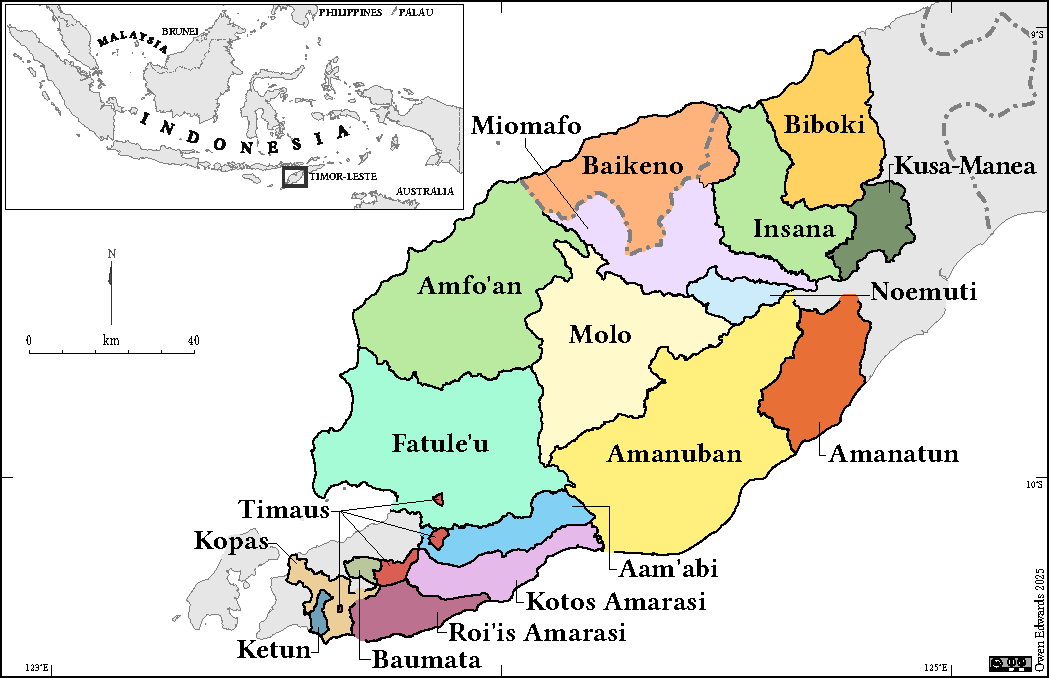
\includegraphics[width=\columnwidth]{figures/Metos}
\end{figure}

\begin{exe}
	\ex{Sources of Meto data in this chapter:}\label{ex:SouMetDat}
 \ea Roi{\Q}is Amarasi, Buraen village, Suit hamlet
					 -- 101 minute corpus of recorded texts \citep{ed14-RoqisParadisec};
	 \ex Kotos Amarasi, Nekmese{\Q} village, Koro{\Q}oto hamlet
					 -- 180 minute corpus of recorded texts \citep{ed09-KotosParadisec};
	\ex Amanuban, Niki-niki village
				 -- elicitation, supplemented by draft Bible translation;{\footnotemark}
				\footnotetext{The (draft) Bible translations into varieties of Meto
							have been carried out by native speakers
							and are completely natural and idiomatic.
							Nonetheless, no analyses or facts presented in this chapter
							are based only on examples found in Bible translations.
							}
		 \ex Amfo{\Q}an, Lelogama village
				 -- 153  minute corpus of recorded texts \citep{cu17-AmfoanParadisec},
				supplemented by \citet{grsuorcu21}, and draft Bible translation; 
		 \ex Timaus, Bokong village, Sanenu hamlet
				 -- 99 minute corpus of recorded texts \citep{ed16-TimausParadisec};
		\ex Baikeno (multiple villages)
				 -- data collected primarily by Charles E. Grimes,{\footnotemark}
						supplemented by translation of the Gospel of Mark.
						\footnotetext{Additional Baikeno data comes from a language documentation workshop
							run by the Endangered Language Alliance in Kupang in July 2012
							during which Edwards was an instructor.}
\z
\end{exe}

Meto varieties have five vowels /i, e, a, o, u/.
Mid vowels phonetically vary between mid-low [ɛ ɔ] and mid-high [e o].
Meto does not have segmental diphthongs.
Sequences of two vowels can be realised as either
vowel-vowel or vowel-glide; e.g. \ve{ai} {\ra} [ˈʔa.i] {\tl} [ʔaj] `fire'.
Every phonological and morphological process of the language
treats phonetically long vowels identically to vowel sequences,
and they are thus analysed as sequences of identical vowels;
e.g. \ve{bif\tbr{ee}} {\ra} \mbox{[bɪˈf\tbr{ɛː}]} `woman'.
See \citet[96--98]{ed20} and \citet[31--32]{ed18-MorphMet}
for further discussion and justification of this analysis.

All (known) Meto varieties have
11 core consonants /p, t, k, ʔ, b, f, s, h, m, n/, as well as either /r/ or /l/
which correspond to one another;
e.g. Kotos, Roi{\Q}is, and Kusa-Manea \ve{koro}, other Meto \ve{kolo} `bird'.
Timaus has both /l/ and /r/ with /l/
corresponding to other Meto /l/ or /r/
and /r/ due to *{dʒ} > \textit{r} (\sectref{sec:TimJ>r}).
In addition to these consonants, most varieties of Meto also have
a voiced palatal obstruent /dʒ/ [dʒ] {\tl} [ʒ]  and a voiced
velar obstruent, either /\gw/ or /g/,
though some varieties lack the voiced velar obstruent.
These obstruents have a restricted distribution
and mainly (though not exclusively) arise due to
the consonant epenthesis which is the focus of this chapter.
Amanuban does not have these obstruents,
but has glides /w/ and /j/ in comparable environments.
The labio-velar obstruent /{\gw}/ is realised
as [ɡw] {\tl} [ɣw], a voiced velar plosive or fricative followed by a labio-velar glide,
or as [ɡ] {\tl} [ɣ], without a following labio-velar glide.
In this chapter we make a distinction in our transcription between 
\textit{<\gw>} = [ɡw] {\tl} [ɣw] and \textit{<g>} = [ɡ] {\tl} [ɣ].

Meto roots have a highly constrained
segmental structure based around a disyllabic foot.\footnote{%
Note that we define the foot as a phonological domain intermediate between the syllable and the
prosodic word \citep{cu22}. In addition to various phonotactic phenomena,
evidence for the foot domain in Meto comes from consonant epenthesis and 
partial reduplication (see \citealt{cu-PhD}). 
We do not assume a relationship 
between the foot and stress, which is not typologically supported \citep{cu22}, and analyse stress in Meto as assigned to the penultimate syllable of the word. There 
is no need to appeal to foot structure to account for the distribution of stress in Meto. See \citet{cu-PhD} for further discussion.} Roots must minimally comprise a foot, and contain a maximum
of two feet. 
Consonant clusters only occur at the juncture of a foot and/or word-initially.
Vowel sequences do not occur across a foot boundary, and all feet
must have an onset consonant. When a word or foot has no onset,
a consonant is automatically inserted (see \sectref{sec:CInsOther}). 
An overview of permitted root structures in Meto with examples 
from Amfo{\Q}an is given in \tabref{tab:RootStucs}.
Words which have more than two syllables are nearly
all historically morphologically complex or are loans.

\begin{table}
\caption{Amfo{\Q}an root structures}\label{tab:RootStucs}
\fittable{\begin{tabular}{ll@{~}c@{~}rlll}
	\lsptoprule
	          & & \multicolumn{1}{c}{Other}    & \\
	Structure & & \multicolumn{1}{c}{material} &Foot&Root & Translation\\ \midrule
	\sub{\wrd}[\sub{Ft}[{\syll}{\syll}]]
	&=	&							&(C)V(C)V(C)& \ve{nima}				& `five' \\
	&   &   					&           & \ve{lalan}			& `path, way' \\
	&   &   					&           & \ve{oef}				& `soup' \\
	\sub{\wrd}[C\sub{Ft}[{\syll}{\syll}]]
	&=	& C						&CV(C)V(C)	& \ve{snaen}			& `sand' \\
	&   &  						&        		& \ve{kninoʔ} 	 	& `clean, holy'\\
	&   &   					&        		& \ve{ʔbaʔu}			& `bat'\\
	\sub{\wrd}[{\syll}\sub{Ft}[{\syll}{\syll}]]
	&=	& (C)V(C)			&CV(C)V(C)	& \ve{maʔfenaʔ}		& `heavy' \\
	&		&							&						&	\ve{maslaal}		& `coarse'\\	
	&		&							&						&	\ve{ansao-n}		& `chest'	\\
	\sub{\wrd}[\sub{Ft}[{\syll}{\syll}]\sub{Ft}[{\syll}{\syll}]]						
	&=	& (C)V(C)V(C)	&CV(C)V(C) 	& \ve{likusaen}		& `python'\\
	&   &         		&        		& \ve{ataʔlaʔe}		& `praying mantis'\\
	&   &        			&        		& \ve{ai{dʒ}iak}	& `jackfruit'\\ 
	\lspbottomrule
	\end{tabular}}
\end{table}

Meto demonstrates acoustic evidence for stress -- specifically from vowel quality, spectral tilt and pitch rise/fall ratios --  on the  penultimate syllable of the word \citep{cu-PhD}. 
Syllable weight is not relevant for any aspect of Meto phonology.
The only roots which do not comprise at least a foot -- i.e. are monosyllabic --  are a small number of functors,
or function morphemes (morphemes with a non-lexical, grammatical meaning). 

Meto has a productive process of final CV {\ra} VC metathesis;
e.g. \ve{hitu} {\ra} \ve{hiut} `seven'.\footnote{The productivity of metathesis is demonstrated by loans undergoing the process,  such
as Malay \ve{kepala} {\ra} \ve{kepaal} `head, chief' (see \citealt[273 ff.]{ed20}).}
The forms and functions of metathesis have been thoroughly
described for Kotos Amarasi by \citet{ed20}, who shows that
in this variety of Meto metathesis has two morphological functions
(modification in the NP and resolution in the discourse)
and is also phonologically conditioned before vowel-initial enclitics.
Most varieties of Meto have assimilation of final /a/ after metathesis,
e.g. \ve{nima} {\ra} \ve{niim} `five', though Kusa-Manea preserves
forms without assimilation, e.g. \ve{niam} `five'.

\section{Overview of the data}\label{sec:Data}
\largerpage
In this section we provide an overview of consonant epenthesis in Meto.
We begin in \sectref{sec:BasFac} with an overview of the basic facts:
when epenthesis occurs and what consonants are inserted.
This is followed in \sectref{sec:InsNotDel} with justification
for analysing this process as epenthesis, not deletion.
In \sectref{sec:Prod} we provide evidence that consonant epenthesis
is a productive process.
In many cases, due to restrictions of space, we cannot fully illustrate
the patterns we discuss here. Wherever insufficient data is provided
to establish that a particular pattern is regular, supporting data
can be found in \appref{sec:AddDat}.

\subsection{Basic facts}\label{sec:BasFac}
Consonant epenthesis --
that is, insertion of consonants which are not present in the phonological
representation (see \sectref{sec:TypBack} below) -- 
occurs in Meto at the juncture
of a vowel-final word and a vowel-initial enclitic. For example,
Amfo{\Q}an \ve{hau} `tree, wood + \ve{=ees} `one, a'
{\ra} \ve{hau{\gw}ees} `a tree'.
The different consonants inserted in this environment
amongst the varieties of Meto we examine
are summarised in \tabref{tab:SummaryInsCs}
according to whether they attach to a host
with final vowel sequence (e.g. \ve{hau} `wood, tree')
or a host with final CV (e.g. \ve{fatu} `stone').

\begin{table}[b]
\centering
\begin{threeparttable}[b]
\caption{Summary of epenthetic consonants in Meto}\label{tab:SummaryInsCs}
	\begin{tabularx}{\textwidth}{Xlccccc ccccc}
	\lsptoprule
	&\multicolumn{5}{c}{VV-final hosts} & \multicolumn{5}{c}{CV-final hosts} \\\cmidrule(lr){2-6}\cmidrule(lr){7-11}
	&	i		&	e		&	a		&	o		&	u		&	i		&	e		&	a		&	o		&	u		\\	\midrule
	Amanuban	&	j	\cellcolor{Pink}	&	j	\cellcolor{Pink}	&	j	\cellcolor{Pink}	&	w	\cellcolor{PaleBlue}	&	w	\cellcolor{PaleBlue}	&	j{\tl}{\0}	\cellcolor{Pink}	&	j{\tl}{\0}	\cellcolor{Pink}	&	{\0}		&	w{\tl}{\0}	\cellcolor{PaleBlue}	&	w{\tl}{\0}	\cellcolor{PaleBlue}	\\	
	Kotos	&	{dʒ}	\cellcolor{Orange}	&	{dʒ}	\cellcolor{Orange}	&	{\gw}	\cellcolor{turquoisegreen}	&	{\gw}	\cellcolor{turquoisegreen}	&	{\gw}	\cellcolor{turquoisegreen}	&	{dʒ}	\cellcolor{Orange}	&	{dʒ}	\cellcolor{Orange}	&	{\0}		&	{\gw}	\cellcolor{turquoisegreen}	&	{\gw}	\cellcolor{turquoisegreen}	\\	
	Roi{\Q}is (Buraen)	&	{dʒ}	\cellcolor{Orange}	&	{dʒ}	\cellcolor{Orange}	&	?\tnote{†}		&	b	\cellcolor{carolinablue}	&	b	\cellcolor{carolinablue}	&	{dʒ}	\cellcolor{Orange}	&	{dʒ}	\cellcolor{Orange}	&	{\0}		&	b	\cellcolor{carolinablue}	&	b	\cellcolor{carolinablue}	\\	
	Baikeno	&	{dʒ}	\cellcolor{Orange}	&	l	\cellcolor{puce}	&	{b}	\cellcolor{carolinablue}	&	b	\cellcolor{carolinablue}	&	b	\cellcolor{carolinablue}	&	{dʒ}	\cellcolor{Orange}	&	{dʒ}	\cellcolor{Orange}	&	{\0}		&	b	\cellcolor{carolinablue}	&	b	\cellcolor{carolinablue}	\\	
	Amfo{\Q}an	&	{dʒ}	\cellcolor{Orange}	&	l	\cellcolor{puce}	&	{\gw}	\cellcolor{turquoisegreen}	&	{\gw}	\cellcolor{turquoisegreen}	&	{\gw}	\cellcolor{turquoisegreen}	&	{dʒ}	\cellcolor{Orange}	&	l	\cellcolor{puce}	&	{\0}		&	{\gw}	\cellcolor{turquoisegreen}	&	{\gw}	\cellcolor{turquoisegreen}	\\	
	Timaus	&	r	\cellcolor{goldenyellow}	&	l	\cellcolor{puce}	&	{\gw}	\cellcolor{turquoisegreen}	&	{\gw}	\cellcolor{turquoisegreen}	&	{dʒ}	\cellcolor{Orange}	&	r		\cellcolor{goldenyellow}	&	l	\cellcolor{puce}	&	{\0}		&	{\gw}	\cellcolor{turquoisegreen}	&	{dʒ}	\cellcolor{Orange}	\\	
	\lspbottomrule
	\end{tabularx}
\begin{tablenotes} \footnotesize
\item [†] Data is lacking for hosts with final /Va/ for Roi{\Q}is from the village of Buraen.
\end{tablenotes}
\end{threeparttable}
\end{table}

\begin{table}[b]
\begin{threeparttable}[b]
\caption{Consonant epenthesis with vowel-initial enclitics  /VV{\gap}}\label{tab:ConInsVowIniCliVV}
\begin{tabularx}{\textwidth}{Xllllll}
	\lsptoprule
				&	`a fire'	&	`a water' 	&	`two already'	&	`a cat'	&	`a tree'	\\
				&	ai=ees	&	oe=ees	&	nua=een\tnote{†}	&	meo=ees 	&	hau=ees	\\	\midrule
	{Amanuban}	&	\ve{ai\tbr{j}ees}	&	\ve{oe\tbr{j}ees}	&	\ve{nua\tbr{j}een}	&	\ve{meo\tbr{w}ees}	&	\ve{hau\tbr{w}ees}	\\
	{Kotos}	&	\ve{aa\tbr{dʒ}ees}	&	\ve{oo\tbr{dʒ}ees}	&	\ve{nua\tbr{\gw}een}	&	\ve{mee\tbr{\gw}ees}	&	\ve{haa\tbr{\gw}ees }	\\
	{Buraen Roi{\Q}is}	&	\ve{aa\tbr{dʒ}ees}	&	\ve{oo\tbr{dʒ}ees}	&	?	&	\ve{mee\tbr{b}oes}	&	\ve{haa\tbr{b}oes}	\\
	{Baikeno}	&	\ve{ai\tbr{dʒ}ees}	&	\ve{oe\tbr{l}ees}	&	\ve{nua\tbr{b}een}	&	\ve{meo\tbr{b}ees}	&	\ve{hau\tbr{b}ees}	\\
	{Amfo{\Q}an}	&	\ve{ai\tbr{dʒ}ees}	&	\ve{oe\tbr{l}ees}	&	\ve{haa\tbr{\gw}een}\tnote{†}	&	\ve{meo\tbr{\gw}ees}	&	\ve{hau\tbr{\gw}ees}	\\
	{Timaus}	&	\ve{aa\tbr{r}ees}	&	\ve{oe\tbr{l}ees}	&	\ve{nua\tbr{\gw}een}	&	\ve{mee\tbr{\gw}ees}	&	\ve{haa\tbr{dʒ}ees}	\\
	\lspbottomrule
\end{tabularx}
\begin{tablenotes} \footnotesize
\item [†] Amfo{\Q}an \ve{haa{\gw}een} is `four already' from \ve{haa} `four'.
Amfo{\Q}an \ve{nuga} `two' is CV-final.
\end{tablenotes}
\end{threeparttable}
\end{table}


An example of each epenthetic consonant is given in
\tabref{tab:ConInsVowIniCliVV} and \tabref{tab:ConInsVowIniCliCV}.
CV-final hosts also undergo metathesis followed by final vowel assimilation
to various extents in different varieties of Meto,
such as Kotos \ve{mo\tbr{ne}} + \ve{=ees} {\ra} \ve{mo\tbr{on}{dʒ}ees} `a husband'
and \ve{fa\tbr{tu}} + \ve{=ees} {\ra} \ve{fa\tbr{at}{\gw}ees} `a stone'.
In Amanuban consonant insertion does
not universally occur after CV-final hosts.
Instead, the host can just undergo metathesis and 
vowel assimilation, and the first vowel of the enclitic
can assimilate to the original final vowel of the host,
e.g. \ve{fa\tbr{fi}} + \ve{=\tbr{e}es} {\ra} \ve{fa\tbr{afi}es} `a pig'.

Whether metathesis and vowel assimilation occur with CV-final hosts
is dependent on a combination of factors including:
the variety of Meto, the phonotactic shape of the host,
and the segments in the final syllable of the host.
There also appear to be speaker and/or
dialect differences in some Meto varieties.
The patterns are complex and not yet
fully understood for all varieties of Meto.



\begin{table}[t]
\centering
\begin{threeparttable}[b]
\caption{Consonant epenthesis with vowel-initial enclitics /CV{\gap}}\label{tab:ConInsVowIniCliCV}
\begin{tabularx}{\textwidth}{Xllllll}
	\lsptoprule
			&	`a pig'	&	`a husband'	&	`gets it'	&	`a day'	&	`a stone'	\\	
			&	fafi=ees	&	mone=ees	&	n-ana=ee	&	neno=ees	&	fatu=ees	\\	\midrule
	Amanuban &	\ve{fafi\tbr{j}ees}	&	\ve{mone\tbr{j}ees}	&	\ve{naanee}	&	\ve{neno\tbr{w}ees}	&	\ve{fatu\tbr{w}ees}	\\	
	Amanuban &	\ve{faafies}	&	\ve{moonees}	&		&	\ve{neenoes}	&	\ve{faatues}	\\	
	{Kotos}	&	\ve{faaf\tbr{dʒ}ees}	&	\ve{moon\tbr{dʒ}ees}	&	\ve{naanee}	&	\ve{neen\tbr{\gw}ees}	&	\ve{faat\tbr{\gw}ees}	\\	
	{Buraen Roi{\Q}is}	&	\ve{faaf\tbr{dʒ}ees}	&	\ve{moon\tbr{dʒ}ees}	&	\ve{naanee}	&	\ve{neen\tbr{b}oes}	&	\ve{faat\tbr{b}oes}	\\	
	{Baikeno}	&	\ve{faaf\tbr{dʒ}ees}	&	\ve{moon\tbr{dʒ}ees}	&	\ve{naanee}	&	\ve{neem\tbr{b}ees}	&	\ve{faat\tbr{b}ees}	\\	
	Amfo{\Q}an &	\ve{fafi\tbr{dʒ}ees}	&	\ve{mone\tbr{l}ees}	&	\ve{naanee}	&	\ve{neno\tbr{\gw}ees}	&	\ve{fatu\tbr{\gw}ees}	\\	
	Amfo{\Q}an	&	\ve{faaf\tbr{dʒ}ees}	&	\ve{moon\tbr{l}ees}	&		&	\ve{neen\tbr{\gw}ees}	&	\ve{faat\tbr{\gw}ees}	\\	
	{Timaus}	&	\ve{faaf\tbr{r}ees}	&	\ve{mona\tbr{l}ees}\tnote{†}	&	\ve{naanee}	&	\ve{neen\tbr{\gw}ees}	&	\ve{faat{dʒ}ees}	\\	
	\lspbottomrule
\end{tabularx}
\begin{tablenotes} \footnotesize
\item [†] Sanenu Timaus has *e > \it{a} /C{\gap}(C){\#}.
\end{tablenotes}
\end{threeparttable}
\end{table}

The vowel-initial enclitics which trigger consonant epenthesis are listed in \tabref{tab:MetVowIniEnc}.
Each of these enclitics can be analysed as a disyllabic foot (see below),
with consonant insertion occurring at the clitic boundary
which is the juncture of two feet.

\begin{table}
	\fittable{
	\begin{threeparttable}[b]
	\caption{Meto vowel-initial enclitics}\label{tab:MetVowIniEnc}
		\begin{tabular}{llll}\lsptoprule
			Form						&Gloss	& Meaning\\ \midrule
			\ve{=ii}				&\tsc{`1det}'	& definite referent near/relevant to speaker\\
			\ve{=ana/=aan}	&\tsc{`2det}'	&	definite referent near/relevant to addressee\\
			\ve{=ee}				&\tsc{`3det}'	& definite referent near/relevant to a third person\\
											&\tsc{`3sg.acc}'	&	third person P argument (object) of verb\\
			\ve{=aa}				&\tsc{`0det}'	&	definite referent near/relevant to no one (≈obviative)\\
			\ve{=esa/=ees}	&`one, a'	&	the numeral one (1); indefinite singular\\
			\ve{=ena/=ee(n)}\tnote{†}	&\tsc{`perf}'	&	perfect, already \\
			\ve{=aha/=aah}		&`just'				&	restrictive\\
			\ve{=oo-n}				&\tsc{`refl}'	& reflexive \\ \lspbottomrule
		\end{tabular}
		\begin{tablenotes} \footnotesize
			\item [†] The perfect enclitic is usually \ve{=ee} in Amfo{\Q}an,
								though sporadic instances of \ve{=ena/=een} are also found.
								Similarly, Baikeno has variation between \ve{=ena} and \ve{=ee}.
								Roi{\Q}is Amarasi has consonant-initial \ve{=hena/=heen}.
		\end{tablenotes}
	\end{threeparttable}
	}
\end{table}

Evidence that these enclitics are
disyllabic comes from two sources.
Firstly, four of these enclitics have unambiguously
disyllabic unmetathesised forms:
\ve{=ana} \tsc{`2det}', \ve{=esa} `one',
\ve{=ena} \tsc{`perf}', and \ve{=aha} `just'.
Consistent with all /a/-final stems
(e.g. \ve{nima} {\ra} \ve{niim} `five'),
final /a/ undergoes assimilation after metathesis
for \ve{=esa} {\ra} \ve{=ees} `one' and \ve{=ena} {\ra} \ve{=een} \tsc{`perf}'
in most varieties of Meto (\sectref{sec:LangBack}),
although assimilation of final /a/ does not occur in Kusa-Manea, e.g. \ve{eas} `one'.

Secondly, in some varieties of Meto there is a process
whereby the initial vowel of a vowel-initial enclitic
undergoes partial assimilation to the quality of the
final vowel of the host.\footnote{This process has been attested in Amanuban,
		Roi{\Q}is Amarasi, and Kopas from Oepaha village.}
Examples from Roi{\Q}is include \ve{nif\tbr{u}} `thousand' + \ve{=\tbr{e}es}
{\ra} \ve{niifb\tbr{o}es} `one thousand',
and \ve{ta-knin\tbr{u}ʔ} `we clean' + \ve{=\tbr{e}e} \tsc{`3sg.acc}'
{\ra} \ve{takniinʔ\tbr{o}e} `we clean it'.
See \citet[248--252]{ed20} for additional examples and discussion.

Despite the evidence that the vowel-initial enclitics
are disyllabic and contain a foot, forms with a sequence
of two identical vowels are frequently realised with a short vowel.
This is a consequence of the stress patterns of Meto.
Stress in Meto is penultimate, but enclitics
are extra-metrical and do not bear stress;
e.g. Amfo{\Q}an \ve{ai} `fire' + \ve{=ees} {\ra} /aidʒees/ [ˈʔaidʒɛs].
Unstressed vowel sequences often have a shorter duration
than stressed vowel sequences in Meto \citep[98--99]{ed20}.

Consonant epenthesis only occurs after vowel-final words.
After consonant-final words, the enclitic is simply attached to the stem.
Thus, all varieties discussed in this chapter have 
\ve{tuaf} `person' + \ve{=ees} {\ra} \ve{tuafees} `a person'
and \ve{sii-t} `song' + \ve{=ees} {\ra} \ve{siitees} `a song', for example.
CVC-final stems similarly do not trigger consonant epenthesis.\footnote{%
In this environment, final CV {\ra} VC metathesis occurs to differing
extents in different varieties of Meto;
e.g. Kotos Amarasi \ve{muʔit} + \ve{=ees} {\ra} \ve{muiʔtees} `an animal'.}

In some cases, the final vowel of a VV-final host undergoes assimilation
to the quality of the previous vowel after consonant epenthesis.
The quality of the vowel before assimilation determines
the type of epenthetic consonant.
This occurs in Kotos, Roi{\Q}is, and Timaus,
after all hosts except hosts with final /Va/ or, in Timaus, /e/,
as seen in \ve{ha\tbr{u}} + \ve{=ees} {\ra} Kotos \ve{ha\tbr{a}{\gw}ees},
Roi{\Q}is \ve{ha\tbr{a}boes}, or Timaus \ve{ha\tbr{a}{dʒ}ees} `a tree'.
See \appref{sec:AddDat} for examples in addition to those in \tabref{tab:ConInsVowIniCliVV}.

Consonant epenthesis is an automatic process which occurs whenever
a vowel-initial enclitic attaches to a vowel-final host,
affecting all morphemes of all word classes without exception,
including other enclitics, as well as new loanwords (see \sectref{sec:Prod} for examples).
Examples of epenthesis with word classes other
than nouns are given in \appref{sec:AddDat}.

The description given above covers nearly all the Meto data.
However, rare combinations of morphemes sometimes have
unexpected patterns of consonant epenthesis.
For example, \citet[244ff]{ed20} describes
the patterns of epenthesis for Kotos Amarasi
when a vowel-initial enclitic attaches to another vowel-initial enclitic.
In this case, unexpected epenthesis of /\gw/ can occur.
Thus, for example, Kotos \ve{oe} + \ve{=ee} \tsc{`3det}' {\ra} \ve{oodʒee} `the water'
has expected insertion of \mbox{/dʒ/} after final /e/.
However, the addition of \ve{=een} \tsc{`perf}' to \ve{oodʒee} `the water'
produces \ve{oodʒee\tbr{\gw}een} `the water already' with
unexpected epenthesis of /\gw/.
In Kotos we would expect /dʒ/ to be inserted after /e/
and would only expect /\gw/ to be inserted after /a/, /o/, or /u/.
Whenever such an unexpected consonant epenthetic consonant
occurs, it corresponds to the default epenthetic consonant (\sectref{sec:Def}).
While it is important to note that such instances do occur,
we do not discuss them further in this chapter as
they are a minor pattern in the language.

\subsection{Epenthesis, not deletion}\label{sec:InsNotDel}
An alternative analysis of the data presented in the previous
section would be to propose that the consonants which appear
before vowel-initial enclitics are part of the stem or enclitic, and are deleted in certain contexts.
They could be analysed as the initial segment of the enclitic,
or they could be analysed as the final segment of the stem.
There is evidence against both analyses.

\hspace*{-3.6pt}Firstly, the consonants which occur before vowel-initial
enclitics are completely predictable based
on the final vowel of the clitic host.
In cases of synchronic deletion, on the other hand,
the quality of the deleted consonants are typically
not phonologically predictable \citep{ha11-delete}.

Secondly, if these consonants are actually the initial
segment of the enclitic, their absence after stems
with final /Ca/ is inexplicable.
Other consonant-initial enclitics 
freely occur with /Ca/-final stems. 
Two examples are Kotos \ve{n-ana} `3-get' + \ve{=kau} \tsc{`1sg.acc'} {\ra}
\ve{naankau} `got me' and
Roi{\Q}is \ve{ku-snasa} `\tsc{1sg}-rest' + \ve{=heen} \tsc{`perf}'
{\ra} \ve{kusnaasheen} `I had rested'.
There are also no restrictions on
clusters involving epenthetic consonants, as shown by forms
such as Kotos \ve{faaf{dʒ}ees} `a pig' or \ve{neen{\gw}ees} `a day'
(among many others in \tabref{tab:ConInsVowIniCliCV}).
There are also roots with initial clusters which involve
the segments which arise in epenthesis.
Examples include Amfo{\Q}an \ve{nguah} [nɡuah] {\tl} [ŋɡuah] `coconut'
and Roi{\Q}is \ve{b{dʒ}ae} [βʒaɛ] `cow'.

Thirdly, if these consonants were the final segment of the stem,
this would entail that they are deleted in all
environments except before a vowel-initial enclitic.
This consonant deletion would occur in a disparate
collection of environments with no clear phonological or phonetic motivation.
It would also be different to other consonant-final words,
such as \ve{tuaf} `person', for which such deletion does not occur.

Furthermore, \citet{mo21} points out that 
plural enclitic allomorphy also supports the analysis of stems
after which consonant epenthesis occurs as vowel-final. This is 
because the plural
enclitic has different forms
 after vowel-final and consonant-final stems. Stems after which consonant epenthesis
occurs do not take the allomorphs found with consonant-final stems.


\begin{table}[b]
	\small
	\caption{Plural enclitic allomorphy}\label{tab:PluEncAll}
 \begin{tabularx}{\textwidth}{Xllll}\lsptoprule
	Stem		&		Kotos		&		Amanuban		&		Amfo{\Q}an		&	Translation		\\	\midrule
\ve{a-pao-t}	&	\ve{apaot=ein}	&	\ve{apaot=eun}	&	\ve{apaot=een}	&	`guards'	\\
\ve{kuan}	&	\ve{kuan=ein}	&	\ve{kuan=eun}	&	\ve{kuan=een}	&	`villages'	\\
\ve{tuaf}	&	\ve{tuaf=ein}	&	\ve{tuaf=eun}	&	\ve{tuaf=een}	&	`people'	\\
\ve{too mfaun}	&	\ve{too mfaun=ein}	&	\ve{too mfaun=eun}	&	\ve{too mfaun=een}	&	`many people'	\\	\midrule
\ve{koro/kolo}	&	\ve{koro=n}	&	\ve{kolo=n}	&	\ve{kolo=n}	&	`birds'	\\
\ve{umi/ume}	&	\ve{umi=n}	&	\ve{ume=n}	&	\ve{ume=n}	&	`houses'	\\
\ve{fafi}	&	\ve{fafi=n}	&	\ve{fafi=n}	&	\ve{fafi=n}	&	`pigs'	\\
\ve{aan feto}	&	\ve{aan feto=n}	&	\ve{aan feto=n}	&	\ve{aan feto=n}	&	`daughters'	\\	\midrule
\ve{hau}	&	\ve{hau=ŋ{\gw}ein}	&	\ve{hau=nuu}	&	\ve{hau=nuug}	&	`trees'	\\
\ve{too}	&	\ve{too=ŋ{\gw}ein}	&	\ve{too=nuu}	&	\ve{too=nuug}	&	`citizens'	\\
\ve{bifee}	&	\ve{bifee=ŋ{\gw}ein}	&	\ve{bifee=nuu}	&	\ve{bifee=nuug}	&	`women'	\\
\ve{oe}	&	\ve{oe=ŋ{\gw}ein}	&	\ve{oe=nuu}	&	\ve{oe=nuug}	&	`kinds of water'	\\
		\lspbottomrule
	\end{tabularx}
\end{table}

\largerpage[-2]
After consonant-final stems, the plural enclitic has a vowel-initial form.
Kotos has \ve{=ein/=eni}, Amanuban has \ve{=eun/=enu}, and Amfo{\Q}an has \ve{=een}.
Examples are given in the first four rows of \tabref{tab:PluEncAll}.\footnote{%
		The plural enclitic after consonant-final stems
		in Roi{\Q}is and Baikeno is \ve{=iin/=ini}.
		Timaus has variation between \ve{=iin/=ini} and \ve{=een}
		for the plural enclitic after consonant final stems.
		Kotos also has sporadic instances of \ve{=enu/=uun} after consonant-final roots.}
However, after vowel-final words the plural enclitic has a different form,
depending on the exact shape of the stem to which it attaches.
After CV-final stems, the plural enclitic is \ve{=n} in all known varieties
of Meto. Examples are given in the middle four rows in \tabref{tab:PluEncAll}.
After stems which end in a vowel sequence (VV-final stems) there is a diversity
of forms: Kotos has \ve{=n{\gw}ein/=n{\gw}eni} [ŋɡwɪn]/[ŋɡwɪni], Amanuban has \ve{=nuu},
and Amfo{\Q}an has \ve{=nuug}.\footnote{%
		Baikeno appears to have \ve{=mbiin/=mbini} after VV-final forms,
		though the Baikeno form requires confirmation.
		The form of the plural enclitic in Buraen Roi{\Q}is and Timaus
		after VV-final forms is currently unknown due to lack of data.
		Kotos has sporadic instances of \ve{=nuu} after VV-final roots \citep[234--244]{ed20}.
		}
Examples are given in the final four rows of \tabref{tab:PluEncAll}.




If the medial consonant in forms such as
Kotos or Amfo{\Q}an \ve{hau{\gw}ees}, or Amanuban \ve{hauwees} `a tree' 
were underlyingly part of the host, we would
expect the plural enclitic to take the forms
found with consonant-final stems: Kotos \textit{*hau{\gw}=ein},
Amanuban \textit{*hauweun}, and Amfo{\Q}an \textit{*hau{\gw}een} `trees'.
That these forms do not occur is evidence that the stems
are underlyingly vowel-final roots.

\subsection{Productivity}\label{sec:Prod}
Consonant epenthesis in Meto is highly productive
and applies to all eligible words.
Vowel-final loans, as well as instances of code-switching, trigger consonant epenthesis.
Examples of such loans/code switches that have entered Kotos Amarasi
via Malay are given in \tabref{tab:ConInsLoa} to illustrate.

\begin{table}
	\small
	\begin{threeparttable}[b]
	\caption{Consonant epenthesis with loans/code switching}\label{tab:ConInsLoa}
		\begin{tabularx}{\textwidth}{Xl@{~}ll@{~}lll}\lsptoprule
Malay	&	&	Kotos	&			&	Output	&	Translation	\\	\midrule
\it{R.T.}\tnote{†}	&	[erte]	&	\ve{erte\tbr{i}}	&	+	\ve{=ii}	&	\ve{ertee\tbr{dʒ}ii}	&	`the R.T. (neighbourhood)'	\\	
\it{H.P.}\tnote{†}	&	[hape]	&	\ve{hape\tbr{i}}	&	+	\ve{=ii}	&	\ve{hapee\tbr{dʒ}ii}	&	`the H.P. (mobile phone)'	\\	
\it{T.V.}	&	[tivi]	&	\ve{tif\tbr{i}}	&	+	\ve{=ii}	&	\ve{tiif\tbr{dʒ}ii}	&	`the TV'	\\	
\it{lemari}	&	[ləmari]	&	\ve{ləmar\tbr{i}}	&	+	\ve{=ii}	&	\ve{ləmaar\tbr{dʒ}ii}	&	`the wardrobe'	\\	
\it{peti}	&	[peti]	&	\ve{pet\tbr{i}}	&	+	\ve{=ii}	&	\ve{peet\tbr{dʒ}ii}	&	`the casket'	\\	
\it{sore}	&	[sore]	&	\ve{sor\tbr{e}}	&	+	\ve{=ii}	&	\ve{soor\tbr{dʒ}ii}	&	`the afternoon'	\\	
\it{penatua}	&	[pənatua]	&	\ve{pentu\tbr{a}}	&	+	\ve{=ii}	&	\ve{pentua\tbr{\gw}ii}	&	`the church elder'	\\	
\it{K.K.}\tnote{†}	&	[kaka]	&	\ve{kaaka\tbr{a}}	&	+	\ve{=esa}	&	\ve{kaakaa\tbr{\gw}esa}	&	`one K.K. (family head)'	\\	
\it{oto}	&	[oto]	&	\ve{ot\tbr{o}}	&	+	\ve{=ii}	&	\ve{oot\tbr{\gw}ii}	&	`the car'	\\	
\it{rokok}	&	[rokoʔ]	&	\ve{rok\tbr{o}}	&	+	\ve{=ii}	&	\ve{rook\tbr{\gw}ii}	&	`the cigarette'	\\	
\it{ibu}	&	[ibu]	&	\ve{ib\tbr{u}}	&	+	\ve{=ii}	&	\ve{iib\tbr{\gw}ii}	&	`the mother'	\\	
\it{sapatu}	&	[sapatu]	&	\ve{sapat\tbr{u}}	&	+	\ve{=ii}	&	\ve{sapaat\tbr{\gw}ii}	&	`the shoes'	\\	
		\lspbottomrule\end{tabularx}
		\begin{tablenotes} \footnotesize
			\item [†] R.T. = \textit{rukun tetangga}, H.P. = \textit{hand phone}, K.K. = \textit{kepala keluarga}
		\end{tablenotes}
	\end{threeparttable}
\end{table}

While some of these examples (e.g. \ve{oto} `car') are probably
loans that have been integrated into the language,
others, such as \ve{ləmari} `wardrobe'
(with unassimilated /l/ and /ə/),\footnote{%
		The foreign segments /l/ and /ə/ would be
		assimilated in Kotos as /r/ and /a/ respectively,
		as seen in examples such as
		Malay /bətul/ → Kotos \ve{batuur} `truly'
		among many others.}
are foreign insertions or instances of code-switching.
Such data shows that consonant epenthesis in Meto
is fully productive and is not morphologically or lexically
restricted to a subset of the lexicon.

\subsection{Consonant insertion in other environments}\label{sec:CInsOther}
Apart from the epenthesis which is the focus of this chapter and was described above, other consonant insertion processes are attested in Meto.
The first is a process of glottal stop epenthesis, which occurs in two environments,
and the second is a process of word-final consonant insertion.

\subsubsection{Glottal stop epenthesis}
Glottal stop epenthesis occurs when a CV- syllable is prefixed to vowel-initial stems.
This process is most clearly exemplified by verb roots which
take consonantal C- agreement prefixes when intransitive 
and syllabic CV- prefixes when transitive.
Examples from Amfo{\Q}an are given in \tabref{tab:GloStpEpe},
with the third person agreement prefixes \ve{n-} or \ve{na-}.
This epenthesis occurs occurs at an affix boundary in the environment /CV-{\gap}V
to resolve hiatus between a prefix and a root.

\begin{table}
\caption{Glottal stop epenthesis: Amfo{\Q}an}
\label{tab:GloStpEpe}
 \begin{tabularx}{\textwidth}{Xlll}
  \lsptoprule
	&	Intransitive	&	Transitive 	&	Translation	\\	\midrule
`rise, get up'	&	\ve{n-fena}	&	\ve{na-fena-b}	&	`raise, get someone up'	\\	
`closed, blocked'	&	\ve{n-ʔekaʔ}	&	\ve{na-ʔekaʔ}	&	`close, block'	\\	
`go up, ascend'	&	\ve{n-sae}	&	\ve{na-sae-b}	&	`put up, lift up'	\\	
`drink'	&	\ve{n-inu}	&	\ve{na-\tbr{ʔ}inu-t}	&	`give a drink to someone'	\\	
`see'	&	\ve{n-ita}	&	\ve{na-\tbr{ʔ}ita-b}	&	`show, make see'	\\	
`see, observe'	&	\ve{n-aila}	&	\ve{na-\tbr{ʔ}aila-b}	&	`cause to face towards'	\\	
`lift'	&	\ve{n-aiti}	&	\ve{na-\tbr{ʔ}aiti}	&	`make lift, raise'	\\	
`run, flee'	&	\ve{n-aena}	&	\ve{na-\tbr{ʔ}aena-b}	&	`make flee'	\\	
  \lspbottomrule
 \end{tabularx}
\end{table}

In Meto, all vowel-initial words undergo
 word-initial glottal stop epenthesis. e.g. Amfo{\Q}an  /iko-n/  [ˈʔikɔn] `tail' and /asug/ [ˈʔasug] `dog'.
That is, there are no phonetically vowel-initial words.\footnote{Given this, some other analysts (e.g. \cite{st96b,mo21})
have analysed all word-initial glottal stops as underlying.}
However, some roots have underlying glottal stops 
which occur in all environments, including after consonantal prefixes.
Examples from Amfo{\Q}an  include \ve{n-ʔekaʔ} `close' (from \tabref{tab:GloStpEpe}),
\ve{n-ʔelah} `remain quiet', and \ve{n-ʔonen} `pray' among many others.

We distinguish between underlying and automatic word-initial glottal stops.
However, for roots which never take a C- prefix the evidence is ambiguous
between whether their initial glottal stop is epenthetic or underlying.
The evidence for automatic word-initial glottal stops
is discussed at more length in \citet{ed17-GlottalStop}.

There are two main pieces of evidence that some
forms have an epenthetic initial glottal stop.
Firstly, words with an initial consonant cluster optionally
have prosthesis of [a] word-initially in some cases
and a glottal stop also occurs before this prosthetic vowel;
e.g. Amfo{\Q}an /bnaog/ {\ra} [ˈbnaɔɡ] {\tl} [ʔaˈbnaɔɡ] `ship',
\mbox{/klulu-f/} {\ra} [ˈkluluf] {\tl} [ʔaˈkluluf] `finger, toe'.\footnote{%
		In our transcriptions the prosthetic vowel is separated by a vertical line;
		e.g. \ve{a|bnaog} `ship' in \tabref{tab:AmfAttMod}.
		}
That a glottal stop occurs before a prosthetic vowel
shows that glottal stop epenthesis is productive word-initially.
Secondly, many instances of an initial glottal stop are epenthetic
from a comparative perspective;
e.g. Proto-Malayo Polynesian *ikuR > /iko-n/ {\ra} [ˈʔikɔn] `tail'
and *asu > /asug/ {\ra} [ˈʔasug] `dog'.

To summarise, glottal stop epenthesis clearly
occurs at affix boundaries in the environment /CV-{\gap}V
and there is also evidence that it occurs word-initially.

\subsubsection{Word-final consonant insertion}
An additional kind of consonant insertion
occurs in some varieties of Meto after a vowel-final
word when it occurs as the last member of the noun phrase (NP).
This includes cases when such words are the only member of the noun phrase,
and thus also includes citation form.\footnote{%
		The citation form is the form given as a translation
		under elicitation and that selected by most native speakers
		as the headword in a dictionary.}
This kind of consonant insertion is known to occur in Amfo{\Q}an,
Timaus, Baikeno, Fatule{\Q}u, Kopas, and some varieties of Molo.\footnote{%
		In Baikeno, Fatule{\Q}u and Molo this consonant insertion
		only occurs after VV-final words.}
This process of NP-final consonant insertion involves the same
consonants as those which occur
before the vowel-initial enclitics.

The root, without any final consonant, occurs before attributive modifiers.
Examples of nouns in citation form and before modifiers
in Amfo{\Q}an are given in \tabref{tab:AmfAttMod}.
See \citet{cu18} for further discussion of this process in Amfo{\Q}an.

\begin{table}
\caption{Amfo{\Q}an attributive modification}
\label{tab:AmfAttMod}
\begin{tabularx}{\textwidth}{Xl@{~}l l@{~}l l l@{~}l}
	\lsptoprule
	\multicolumn{2}{l}{Citation form}	&	\multicolumn{2}{l}{Modifier}	&		&	\multicolumn{2}{l}{Phrase} \\ \midrule
	\ve{sisi\tbr{dʒ}}	&	`meat'	&	\ve{metoʔ}	&	`dry'	&	\ra	&	\ve{sisi metoʔ}	&	`dried meat'	\\
	%\ve{fafi\tbr{dʒ}}	&	`pig'	&	\ve{hao-t}	&	`feed'	&	\ra	&	\ve{fafi hao-t}	&	`pig feed'	\\
	\ve{atoni\tbr{dʒ}}	&	`man'	&	\ve{munif}	&	`young'	&	\ra	&	\ve{atoni munif}	&	`young man'	\\
	\ve{bidʒae\tbr{l}}	&	`cow'	&	\ve{fuidʒ}	&	`wild'	&	\ra	&	\ve{bi{dʒ}ae fui{dʒ}}	&	`wild cow'	\\
	\ve{ume\tbr{l}}	&	`house'	&	\ve{bubuʔ}	&	`wild'	&	\ra	&	\ve{ume bubuʔ}	&	`round house'	\\
	\ve{a|bnao\tbr{g}}	&	`ship'	&	\ve{kolog}	&	`bird'	&	\ra	&	\ve{bnao kolog}	&	`aeroplane'	\\
	\ve{neno\tbr{g}}	&	`day'	&	\ve{a-hunu-t}	&	`first'	&	\ra	&	\ve{neno ahunut}	&	`first day'	\\
	\ve{asu\tbr{g}}	&	`dog'	&	\ve{anaʔ}	&	`small'	&	\ra	&	\ve{asu anaʔ}	&	`puppy'	\\
	\ve{kulu\tbr{g}}	&	`teacher'	&	\ve{feʔug}	&	`new'	&	\ra	&	\ve{kulu feʔug}	&	`new teacher'	\\
	\lspbottomrule
\end{tabularx}
\end{table}

It is not possible to analyse this process of consonant insertion
as the same process which is the focus of this chapter. This is because
the two processes occur in different environments and affect different words.
The NP-final consonant insertion is not phonologically predictable
but is determined by the syntactic position of a given word
and primarily affects nouns.\footnote{%
		Verbs with an unexpressed object can
		also have final consonant insertion \citep[39ff]{cu18}.}
On the other hand, epenthesis before vowel-initial enclitics
occurs in a specific phonological environment
and affects all words regardless of word class.
Additionally, epenthesis before vowel-initial enclitics
takes place in varieties of Meto
which do not have NP-final consonant insertion,
such as Amanuban, Kotos, and Roi{\Q}is. 

\section{Typological and theoretical context}\label{sec:TypBack}
This section provides relevant  typological and theoretical context for the 
Meto data outlined in \sectref{sec:Data}.
It   provides an overview of 
how epenthesis has been defined in the literature, 
showing that Meto can be considered a legitimate case of epenthesis (\sectref{sec:DefineEp}).
It then surveys attested epenthetic consonants (\sectref{sec:AttestedCs}),
demonstrating  that the epenthetic consonants attested in Meto are of typological interest.
 It then surveys how consonant epenthesis patterns
have been accounted for (\sectref{sec:TypExplain}, \ref{sec:DefineAsimEp}).

\subsection{Defining epenthesis}\label{sec:DefineEp}
Defining what exactly constitutes consonant epenthesis has been 
an topic of considerable discussion.
Cases of ``minimal" epenthesis -- that is, considered to be minimally disruptive of 
transitions between vowels --  such as insertion of 
glides to resolve hiatus, or insertion of glottal stops at prosodic boundaries,
are widely accepted to be epenthesis.
There are various cases, however, where there has been considerable
discussion as  to whether a given pattern is actually epenthesis, such as 
``intrusive \emph{r}'' in various varieties of English
(see \citealt{vasa17} and \citealt{mo17} for overviews),
/t/ insertion in Ajyíninka Apurucayali (Arawakan, Peru, see \citealp{lo02, dl06, st15, mo15}),
and /g/ insertion in Buriat (Mongolic, Russia/Mongolia/China, see \citealp{mo15, vasa17, st14, st20}).


Such discussions have arisen, in part, due to different
restrictions on what is defined as epenthesis.\footnote{%
		The likelihood that a given pattern is considered to be epenthesis also
		appears to be theoretically motivated. For example, there has been wide
		acceptance of /t/ insertion in Ajyíninka Apurucayali as a case of 
		epenthesis (e.g. \citealt{mc02, dl06}),
		because a coronal consonant would be relatively unmarked under
		an Optimality Theory framework. 
		Buriat /g/ insertion, on the other hand, has not been widely accepted as a 
		legitimate case of epenthesis, and /g/ is a highly marked epenthetic consonant within
		an Optimality Theory framework.  However, 
		\citet[117]{mo08} demonstrates that the evidence for either of these processes being legitimate 
		cases of epenthesis  is, in fact,  comparable.}
An overview of the criteria proposed in the literature is given in \REF{ex:EpenthesisCrit}.


\begin{exe}
\ex Different criteria of epenthesis proposed in the literature:\label{ex:EpenthesisCrit}
	\begin{xlist}
	\ex{occurs in a phonological environment, not morphologically restricted \citep{lo02, dl06, mo15};}
	\ex{is the only process in given phonological context \citep{lo02, dl06},}
	\ex{shows evidence of being synchronically active \citep{mo15};}
	\ex{epenthetic segment is invariant  \citep{lo02, dl06, mo15}.}
	\end{xlist}
\end{exe}

Requirement (\ref{ex:EpenthesisCrit}a) makes explicit that epenthesis must be a phonological process. This excludes
cases of  morphologically conditioned consonant insertion  which have 
sometimes been included in the epenthesis literature. An example is /ɾ/ insertion
in Anejom̃  (Austronesian, Vanuatu), which has often been included
in discussions of epenthesis (e.g. \citealp{vasa17}),
but is limited to compounds, see \citet[186]{st14}. 

\largerpage
Requirement (\ref{ex:EpenthesisCrit}b) refers to a requirement that
no other process occurs in the context where epenthesis occurs.
This excludes instances where consonant epenthesis
is one of several attested hiatus resolution 
strategies. For instance in Rutooro (Atlantic-Congo, Uganda, \citealp{bi21}),
hiatus resolution is achieved by either consonant insertion,
deletion, or diphthongisation. 
Which  process occurs depends on the quality of the vowels.
Consonant insertion in Rutooro would not be considered
a legitimate case of epenthesis according 
to criterion (\ref{ex:EpenthesisCrit}b). 
								
Requirement (\ref{ex:EpenthesisCrit}c) specifically excludes cases
where a consonant process may have been
productive in the past, but is no longer productive.
An example is dorsal insertion in Buriat (Mongolic),
which has sometimes been included in the epenthesis literature,
but does not show evidence of being synchronically productive \citep{st20}.
A requirement by \citet{mo15} is to exclude patterns where less than
65\% eligible morphemes participate,
to ensure that the epenthesis pattern is robust. 

Requirement (\ref{ex:EpenthesisCrit}d) excludes cases of assimilatory epenthesis
in which the quality of the epenthetic
segment varies according to the adjacent vowels \citep[79]{dl06}.
When this criteria has been proposed, this does not   
mean that cases of assimilatory epenthesis are excluded
entirely from being considered cases of epenthesis.
Instead, it is to limit discussions to cases of  default epenthesis
-- the invariable insertion of one segment --
which are of greater theoretical interest.
Default and assimilatory epenthesis are discussed in detail
in \sectref{sec:TypExplain}. 

According to the
different criteria in \REF{ex:EpenthesisCrit}, 
consonant insertion in Meto 
is a legitimate case of epenthesis. It occurs in 
a phonological environment (hiatus at the boundary of two feet, criteria \ref{ex:EpenthesisCrit}a) 
and   is the only process attested to resolve hiatus in this environment (criterion \ref{ex:EpenthesisCrit}b). 
It is synchronically productive (criterion \ref{ex:EpenthesisCrit}c). 
In most cases, the quality of the inserted 
consonant is determined by the previous vowel,
 and thus does not fulfill criterion (\ref{ex:EpenthesisCrit}d).
However, there are some instances in 
Meto which can be classified as  default epenthesis. 
	See \sectref{sec:SyncAccount} for detailed discussion of this matter. 
	
\subsection{Attested epenthetic consonants}\label{sec:AttestedCs}
\largerpage
The most common epenthetic  consonants in hiatus position 
are glides (especially homorganic glides),
laryngeal consonants, and, more rarely, rhotics /ɹ/, /r/
and coronal consonants such as /t/ \citep{dl06, ca11}.
Of these, insertion of glides is by far
the most widely attested \citep{pi03, uf07, ca11}. 

Several of the  epenthetic  consonants attested in Meto, namely \mbox{/dʒ/,} /b/, and \mbox{/\gw/},
have not been previously attested among accepted cases of epenthesis. 
These consonants have also not been reported for any cases where it is contested 
as to whether epenthesis is the best analysis,
with the exception of possible insertion of /g/ in Buriat,
in which case the process is highly disputed (see \sectref{sec:DefineEp}). 
Epenthesis of /l/, which is attested in Meto,
has been reported for several varieties of English (e.g. \citealt{gi02, gi99, ki10}).
However, none of these instances have been shown to be robust patterns \citep[7]{st14}.
Therefore, that Meto attests robust epenthesis of /l/ is also of typological interest. 
 							
\subsection{Explaining the typology of epenthetic consonants}\label{sec:TypExplain}
The common occurrence of certain consonants, such as glides, in epenthesis processes,
and the non- or rare  occurrence of others, has been accounted for by appealing to a
number of factors. 

Articulatory and perceptual factors,
as well as phonetic ``naturalness'', have been 
used to explain the common occurrence of glides and laryngeal consonants epenthetically  \citep{bl08-unnatural}.
For example, epenthesis of /j/ after /i/ in hiatus
can arise from gestural overlap. 
Similarly, from a perceptual perspective,
insertion of /j/ between /i/ and  another vowel could be
explained in terms of /j/  not being particularly 
perceptually salient to hearers in this context, as it does not 
require significant articulatory changes
in the transition from /i/ to the following vowel \citep{st09,mo12}.

There are also various theoretical accounts of attested epenthetic consonants, 
as well as predictions about 
possible epenthetic consonants. These accounts typically rely on a 
distinction between ``default'' and ``non-default'' or
``assimilatory'' epenthesis (e.g. \citealt{dl06,mo12,dlki13}). 
In cases of default epenthesis, one segment is
invariably inserted in a particular phonological environment. For example,
many languages attest default epenthesis of /ʔ/ before
vowel-initial words. Examples include
Maltese \citep{mikich19},
Czech \citep{sipoch12}, and Meto (see \sectref{sec:CInsOther}).
On the other hand, in cases of assimilatory epenthesis, the quality of the epenthetic segment
varies and can be analysed as determined by the place and manner of
articulation of the adjacent vowels \citep[79]{dl06}. 
Typical examples include /j/ as the epenthetic consonant
after front vowels and /w/ after back vowels. 
Examples of languages with this kind of epenthesis abound.
Two examples are Woleaian (Austronesian, Federated States of Micronesia, \citealp{so75})
and Cantonese (Tibeto-Burman, China, see \citealp{ha72}).
Some languages demonstrate both default and assimilatory epenthesis,
such as epenthesis of /j/ and /w/ next to high vowels, 
and epenthesis  of /ʔ/ next to other vowels.
Examples of languages which demonstrate
this kind of epenthesis pattern include Kalinga
(Austronesian, Philippines, see \citealt{ge70}) and Malay \citep{ah05}. 
In some cases for Meto, the inserted segments vary depending
on the quality of the vowel and can be considered as instances of
assimilatory epenthesis (\sectref{sec:SpreadAcc}).
In other cases, however, /j/, /b/ or /\gw/ is the default
inserted consonant (\sectref{sec:Def}). 

Default epenthesis has received considerable attention in the theoretical literature. 
This is because in an Optimality Theory framework
the quality of default epenthetic consonants is
expected to be determined by markedness \citep{mcpr94,lo02,dl06}.  
``Markedness'' in phonology typically refers to a preference for 
certain kinds of structures which are ``unmarked'' (higher frequency, less complex, less phonetically difficult) over others
which are more ``marked'' \citep{mc02,dl06}.\footnote{%
		Markedness is used in many 
		other senses, see \citet{ha06}, \citet{by11} and \citet{hu11}. 
		For an overview of the differences between 
		the use of markedness in Optimality Theory in comparison to other contexts
		see \citet[15]{mc02}.}
In Optimality Theory, epenthesis is considered to be one of several kinds of ``repairs'' that 
phonological inputs can undergo to make them less marked.
For example, consonant epenthesis results in syllables with onsets,
which are considered to be less marked than onsetless syllables \citep{dl06}.
It  is also expected that the quality of the epenthetic consonant which 
resolves hiatus is optimal with
respect to markedness constraints, that is, minimally marked \citep{lo02,dl06,ca11}. 
What exactly makes a consonant more or less marked is debated.\footnote{%
		Markedness has been defined, for example,
		on the basis of articulatory factors \citep{arpu94},
		perceptual factors \citep{st09},
		and abstract factors such as implicational relationships \citep[15]{mc02}.}
 However, the general assumption is that inherent properties of
synchronic phonology play a role in determining the quality of epenthetic consonants
 -- in particular, that, all else being equal,
the epenthetic consonant employed by a language
will have the universally least marked place of articulation \citep{lo02,bl08,ca11}. 
Various hierarchies of consonant place of articulation markedness have been proposed, 
(e.g. \citealt{ke75,papr91}, \citealt[4]{lo02}, \citealt[2]{dl06}).
All rank labial and dorsal consonants as more marked than coronal and glottal.
This predicts a universal preference for coronal and glottal consonants and 
avoidance of labial and dorsal consonants.
Some have gone so far as to predict that labial and  dorsal consonants 
are not  possible epenthetic segments (e.g. \citealt[82]{dl06}). 
However, labial and  dorsal consonants /\gw/ and \mbox{/b/} are attested 
default epenthetic segments in Meto (see \sectref{sec:Def}). 

Proposals about markedness and consonant epenthesis 
are not without controversy. 
Various linguists have questioned the claim that any
particular place of articulation is universally unmarked (e.g. \citealp{hu03,ri07,ri11}).
More broadly, Optimality Theory proposals about preferred epenthetic segments 
have been found not to be borne out cross-linguistically \citep{mo15,vasa17}.  
There is also controversy regarding markedness
as an explanation  of phonological patterns.
This is because there are examples of sound patterns
contradicting markedness claims (see \citealt[183]{hu05} for examples).
Moreover, sound patterns attributed to markedness
can be accounted for by reference to phonetics,
language use, language change \citep{by01,by11,bl04}   
or frequency effects and predictability \citep{hu05}. 

Another way that consonant epenthesis patterns 
have been explained is by
examining their diachronic sources.
\citet{bl08} proposes that ``natural'' or ``minimal''
consonant insertion processes, like intervocalic glide epenthesis,
reflect the phonologisation of earlier phonetically
conditioned sound change.
On the other hand, ``unnatural'' patterns can be accounted for as 
the result of multiple changes,
such as intervocalic glide epenthesis undergoing 
subsequent glide fortition,
or reanalysis of a deleted consonant as being epenthetic \citep{bl08}. 
We observe these same kinds of  sound changes in Meto, which have resulted
in the consonant insertion patterns attested.
The diachronic approach has the potential to
provide us with insights not offered by synchronic accounts (see \sectref{sec:DiacAcc}).

\subsection{Synchronic accounts of assimilatory epenthesis}\label{sec:DefineAsimEp}
In Meto, which consonant 
is inserted is usually determined
by the quality of the previous vowel,
and the process  can therefore be considered assimilatory epenthesis.
However, the inserted consonant is similar to the preceding vowel to differing extents. 
Insertion of /j/ after front vowels and /w/ after back vowels 
in Amanuban can be straightforwardly 
analysed as maximally similar to the surrounding vowels.
Similarly, other inserted consonants (such as /l/ after /e/ in Amfo{\Q}an)
can also be identified as sharing similar features (\cite[51]{cu18}, \cite{mo21}).
However, what features are shared between the vowel
and epenthetic consonants in other cases
(such as insertion of /r/ after /i/ in Timaus) is unclear.


Cases of assimilatory epenthesis documented in the literature
involve insertion of glides, 
[ʋ], [v], [ʝ] \citep[72]{mo12}, and [ɣ] \citep[80]{dl06}.
In such cases, the quality of the inserted segments is
typically explained in terms of sharing features
with the surrounding vowels. 
For example, \citet[56]{st14} proposes that 
/ʋ/ after /oː/ in Dutch occurs because it is 
featurally similar to the vowel
in terms  backness and height  (being non-high). Similarly,
\citet[80]{dl06} proposes that epenthesis
of [ɣ] in Brahui (Dravidian, South Asia) after low back vowels is motivated by 
assimilation to the vowels in terms of dorsality, voice, and continuancy. 

Cases of assimilatory epenthesis which involve 
segments other than glides have also been 
also accounted for in terms of allophony.
For example, \citet[78]{st14} accounts for 
insertion of [ʝ] and [v] in Kalaallisut (Eskimo-Aleut, Greenland) as a result of allophony.
In Kalaallisut, [j, w] and [ʝ, v]  are in complementary distribution.
The glides [j, w] only appear after [i, u],
while the fricatives [ʝ, v] occur in other environments.
Under this analysis, the actual inserted consonant is /j/ or /w/  -- which 
is most featurally similar to /i/ or /u/, but can be realised as [ʝ] or [v] in 
certain contexts.\footnote{%
		For Meto, it is not possible to propose that
		[\gw], [b] or [dʒ] are allophones of glides.
		This is because varieties of Meto with these
		obstruents do not have glides (\sectref{sec:LangBack}).}

Aside from these examples,
the synchronic analysis of assimilatory epenthesis has received considerably
less attention than that of default epenthesis.
One issue which has not been addressed is 
the extent to which a given inserted consonant needs to be similar to surrounding vowels in order be 
considered a case of assimilatory epenthesis; no cut-off point has been proposed.

Returning to the case of Meto,
we could potentially 
propose a cut-off point for how similar to the conditioning 
vowels a epenthetic consonant needs to be in order to be considered assimilatory epenthesis. 
However, the different epenthetic consonants exist on a spectrum.
Some patterns are highly assimilatory (e.g. Amanuban), while others are less assimilatory (e.g. Timaus).
Proposing such a cut-off point would draw an arbitrary
distinction between processes which otherwise
demonstrate the same synchronic behaviour. 
As result, we do not draw a cut-off point in our  discussion of 
how to analyse the Meto data synchronically (\sectref{sec:SyncAccount}).
We also 
demonstrate how this  spectrum of more and less assimilatory 
consonants has arisen as the result of various diachronic changes (\sectref{sec:DiacAcc}).

\section{Synchronic accounts of  Meto consonant epenthesis}\label{sec:SyncAccount}
In this section we briefly outline some of the ways
in which Meto consonant epenthesis
has been analysed from a synchronic perspective.
There are two patterns of consonant epenthesis.
Most epenthetic consonants are determined by the previous vowel
and have been analysed as resulting of feature spreading (\sectref{sec:SpreadAcc}),
while epenthesis after hosts with final /Va/ has not been
analysed as determined by the final vowel of the host
and instead involves default epenthetic consonants (\sectref{sec:Def}).

\subsection{Assimilatory epenthesis: Spreading analysis}\label{sec:SpreadAcc}
In most cases in Meto, the quality 
of the inserted segment is determined by the preceding vowel, and can be considered a process  
of assimilatory epenthesis as defined in the literature (\sectref{sec:TypBack}). 
Assimilatory epenthesis in Meto has
been analysed within Autosegmental Phonology
\citep[215--233]{ed20}, Optimality Theory \citep{mo21},
as well as a combination of both \citep[48--57]{cu18}.
While these accounts differ in many details,
they all draw on the notion that consonant epenthesis results,
at least in part, from the
place and/or manner
features of a vowel spreading onto a 
consonant which does not have any pre-defined features.
This follows other accounts of assimilatory
epenthesis (\citealp{dl06,st14}, see also \sectref{sec:DefineAsimEp})
and is based on the assumption that the quality of the
inserted consonant is determined by the features it shares with with a preceding vowel. 
 
For example, under a spreading 
analysis, \tsc{[+labial]} spreads after /o/ and /u/
in Baikeno and Buraen Roi{\Q}is to yield /b/.
However, in other varieties, a spreading analysis would entail that both 
\tsc{[+labial]} and \tsc{[+velar]}
spread to yield /w/ (Amanuban) or /\gw/ (Kotos, Amfo{\Q}an).
While variations on the spreading analysis can be invoked,
the reasons for why different features spread in different varieties is not fully explained.

The Timaus data, however, present a challenge for the spreading analysis.
Epenthesis of /l/ after /e/ can be analysed by proposing
that both are \tsc{[+coronal, -high]} \citep[51]{cu18} or 
\tsc{[+coronal, -dorsal]} \citep{mo21}.
Similarly, /\gw/ and /o/ are both labio-velar, and 
thus the insertion of /\gw/ after /o/ can be attributed to these features spreading. 
However, it is difficult to account for epenthesis of 
\mbox{/r/} after \mbox{/i/} as a result of feature spreading.
It is especially difficult to identify
features which could spread to result in epenthesis of \mbox{/dʒ/} after \mbox{/u/} 
 -- particularly given epenthesis of \mbox{/\gw/} after \mbox{/o/}. 

\subsection{Default epenthesis}\label{sec:Def}
Default epenthesis  occurs after stems with final /Va/.
The epenthetic consonants inserted after such stems are
summarised in \REF{ex:DefEpe} below.

\begin{exe}
\ex{Epenthesis after hosts with final /Va/:}\label{ex:DefEpe}
	\begin{xlist}
		 \exi{(a)}{epenthesis of /j/ /Va{\gap}=V (Amanuban);}
		 \exi{(b)}{epenthesis of /b/ /Va{\gap}=V (Baikeno);}
		\exi{(c)}{epenthesis of /\gw/ /Va{\gap}=V (Kotos, Amfo{\Q}an, Timaus).}
	\end{xlist}
\end{exe}

The reason that the spreading analyses cannot be readily
extended to cover such cases is because epenthesis does
not occur after stems with final /Ca/.
E.g. Kotos \ve{nua} + \ve{=een} {\ra} \ve{nua{\gw}een} with epenthesis
contrasts with \ve{n-ana} + \ve{=ee} {\ra} \ve{naanee} `gets it' without epenthesis.
If spreading (e.g. of \tsc{[+low]} and/or \tsc{[+voice]})
were at play after stems with final /a/,
the lack of epenthesis after stems with final /Ca/ is unexplained.
This indicates that epenthesis of these consonants after /Va/
is not conditioned by the previous vowel.

Recall from \sectref{sec:TypBack} that typically a binary distinction is made 
between two kinds of epenthesis: assimilatory and default. The former is typically defined as cases 
where surrounding vowels determine the quality of the epenthetic consonant. 
In the case of the latter, they do not.
On this basis, epenthesis after /Va/ could
be considered a case of default epenthesis.

This proposal  -- that there is default epenthesis of 
consonants at enclitic boundaries after certain vowels  --
gains some support from the variety of Kotos Amarasi spoken
in Fo{\Q}asa{\Q} hamlet. In this variety of Meto, /g/
(not labio-velar /\gw/) is inserted after all
vowel-final hosts before an enclitic,
except when the host ends in /Ca/,
in which case epenthesis is optional.
Examples are given in \tabref{tab:FoqConIns}.

\begin{table}
	\caption{Fo{\Q}asa{\Q} consonant epenthesis \citep[232]{ed20}}\label{tab:FoqConIns}
	\begin{tabularx}{\textwidth}{Xrclll}\lsptoprule
	Stem		&		&		Enclitic	&			Fo{\Q}asa{\Q}						&	Translation	\\	\midrule
\ve{umi}	&	+	&	\ve{=ee}	&	\ve{uimgee}					&	`the house'	\\	
\ve{peti}	&	+	&	\ve{=ee}	&	\ve{peitgee}					&	`the casket'	\\	
\ve{n-rari}	&	+	&	\ve{=ee}	&	\ve{nrairgee}					&	`finishes it'	\\	
\ve{n-soʔi}	&	+	&	\ve{=ee}	&	\ve{nsoiʔgee}					&	`counts it'	\\	
\ve{fee}	&	+	&	\ve{=ee}	&	\ve{feegee}					&	`the wife'	\\	
\ve{n-moʔe}	&	+	&	\ve{=ee}	&	\ve{nmoeʔgee}					&	`does it'	\\	
\ve{hau}	&	+	&	\ve{=ii}	&	\ve{haugii}					&	`the tree'	\\	
\ve{neno}	&	+	&	\ve{=ees}	&	\ve{neoŋgees}					&	`one day'	\\	
\ve{na-ʔura}	&	+	&	\ve{=een}	&	\ve{naʔuureen {\tl} naʔuurgeen}					&	`has started raining'	\\	
\ve{n-sosa}	&	+	&	\ve{=ee}	&	\ve{nsoosee {\tl} nsoosgee}					&	`buys it'	\\	
		\lspbottomrule
	\end{tabularx}
\end{table}

\citet{mo21} reports nearly identical data for
Kotos Amarasi from the village Oekabiti 
and analyses it as spreading of \tsc{[+voice]}
with epenthesis of the place and manner features,
with the least marked place/manner being selected.\footnote{%
		See \citet{mo21} for details on how /g/ is determined to be
		the consonant with the least marked place and manner features.}
Whatever the exact analysis, the data presented in this section
demonstrates that some kind of
default epenthesis occurs at clitic boundaries.

Given the evidence for default epenthesis,
an alternative synchronic analysis
of the different epenthetic consonants
might be to propose that the default 
consonant is inserted in all instances
and changes according to the quality of the preceding vowel. 
This would be very similar to the analysis
of Kalaallisut discussed in \sectref{sec:DefineAsimEp}.
Thus, for instance, we could propose that in Amfo{\Q}an
\mbox{/\gw/} {\ra} [l] /e{\gap} and \mbox{/\gw/} {\ra} [dʒ] /i{\gap}.
While \mbox{/\gw/} {\ra} [dʒ] /i{\gap} might be reasonable,
\mbox{/\gw/} {\ra} [l] /e{\gap} is questionable due to
the lack of phonetic similarity between the two consonants.
Furthermore, for Timaus, statements such as \mbox{/\gw/} {\ra} [r] /i{\gap}
or \mbox{/\gw/} {\ra} [dʒ] /u{\gap} lack any clear phonetic
motivation for the realisations proposed.
This analysis also runs into problems for Baikeno,
as [b] is attested after front vowels in all varieties of Meto.
Examples from Baikeno include \ve{na-ʔebok} `ignore', \ve{na-ʔnae-baʔ} `make great',
\ve{bibi} `goat', and \ve{mi-baʔe} `you (pl.) play'.

\section{Diachronic account of Meto epenthesis}\label{sec:DiacAcc}
The main problem faced by synchronic accounts of
consonant epenthesis in Meto is that they do not explain the diversity of consonants
inserted in different varieties of Meto.
Under the analyses that have been proposed, there is no clear motivation as to why certain
features spread in some varieties but not others. 
A diachronic perspective allows us to gain a much
more cohesive and unified explanation for the diversity
of epenthetic consonants; the different consonants
are the result of sound changes
applying to different extents in each variety of Meto.

In this section we outline how the different consonant epenthesis
processes in Meto have developed from a diachronic perspective.
Most of this section is focused on cases where the quality of 
the epenthetic consonant is determined by the final vowel of the clitic host.
The development of default epenthesis
is discussed in \sectref{sec:DevDefIns}.
All Proto-Malayo-Polynesian (PMP) reconstructions found in this section
are from \citet{bltr} and all Proto-Rote-Meto (PRM) reconstructions
are from \citet{ed21-RMDict}.

The series of sound changes that
have occurred after front and back vowels
are summarised in \REF{ex:EpeFroVow} and \REF{ex:EpeBacVow} respectively below.
Each variety of Meto discussed in this chapter
has carried out each series of sound changes in \REF{ex:EpeFroVow} and \REF{ex:EpeBacVow}
to different extents. 

\begin{exe}
	\ex{/V\tsc{[+front]}{\gap}=V \hspace{3mm} {\0} > \it{j} > \it{dʒ} > {{$\left\{\hspace{-1mm}\begin{array}{l}{\textrm{\hp{(*}\it{r}}}\\{\textrm{(*r >) \it{l} /e{\gap} (or direct *j > \it{l})}}\\\end{array}\hspace{-1mm}\right.$}}}\label{ex:EpeFroVow}
	\ex{/V\tsc{[+back]}{\gap}=V \hspace{5.1mm} {\0} > \it{w} > \it{\gw} > {{$\left\{\hspace{-1mm}\begin{array}{l}{\textrm{\it{\hp{*}b}}}\\{\textrm{*g > \it{dʒ} /u{\gap}}}\\\end{array}\hspace{-1mm}\right.$}}}\label{ex:EpeBacVow}
\end{exe}

\subsection{Glide insertion}\label{sec:GliIns}
The first change is glide insertion,
whereby a process of phonetic insertion of [j] and [w] to
resolve hiatus underwent phonologisation.
This kind of phonologisation of a glide insertion process is 
widely attested cross-linguistically (see \citealt[4-6]{bl08}).
This change alone yielded the epenthesis seen in Amanuban.
Phonetic insertion of glides is also attested 
word-medially after high vowels,
but does not usually occur after mid vowels.
Two examples from Amanuban are
\ve{ue} {\ra} [ˈʔuwɛ] {\tl} [ˈʔʊɛ] `rattan',
and \ve{bia} {\ra} [ˈbija] {\tl} [ˈbia] `cow'.

\subsection{Glide fortition}\label{sec:GliFor}
The next stage in the development of consonant epenthesis
is glide fortition, given in \REF{ex:GliFor} below.
These changes affect all varieties of Meto examined in this
chapter except Amanuban.  

\begin{exe}
\ex{Glide fortition:}\label{ex:GliFor}
	\begin{xlist}
		\ex{*j > \textit{dʒ}}
		\ex{*w > \textit{\gw}}
	\end{xlist}
\end{exe}

Glide fortition also occurs word-medially to
different extents in many varieties of Meto.
Examples from Kotos, Amfo{\Q}an, and Baikeno
are given in \tabref{tab:WorMedGliFor} alongside
Amanuban cognates which usually retain a glide,
as well as available PMP and PRM reconstructions
which show that these glides were originally automatic transition glides.

\begin{table}
	\caption{Word-medial glide fortition}\label{tab:WorMedGliFor}
	\begin{tabularx}{\textwidth}{Xllllll}\lsptoprule
PMP&*duha&*ia&*laqia&---&*kahiw+*qaRuhu\\
PRM&*dua&*ia&*laia&---&*kaiou\\\midrule
Amanuban&\ve{nuaʔ}&\ve{ia, ii}&\ve{nai\tbr{j}eeʔ}&\ve{bia, bie}&\ve{ʔa\tbr{i}oo, ʔa\tbr{j}oo}\\
Kotos&\ve{nua}&\ve{ia, i\tbr{dʒ}a}&\ve{nai\tbr{dʒ}eer}&\ve{bi\tbr{dʒ}ae}&\ve{ʔai\tbr{dʒ}oʔo}\\
Amfo{\Q}an&\ve{nu\tbr{g}a}&\ve{i\tbr{dʒ}a, i\tbr{dʒ}e}&\ve{nai\tbr{dʒ}ee-l}&\ve{bi\tbr{dʒ}ae-l}&\ve{ʔai\tbr{dʒ}ao-g}\\
Baikeno&\ve{nu\tbr{b}an}&\ve{i\tbr{dʒ}e}&\ve{}&\ve{bi\tbr{dʒ}ae-l}&\ve{}\\
gloss&`two'&`here'&`ginger'&`cow'&`casuarina'\\
		\lspbottomrule
	\end{tabularx}
\end{table}

Glide fortition is a fairly well-attested change cross-linguistically
and many examples similar to that posited for Meto occur in other Austronesian languages.
Examples include Chamorro \citep[87]{bl00},
many languages of the Aru Islands (\cite[127--133]{co82}, \cite[55]{bl14}, \cite{ni17}),
several languages of Borneo
(\cite[73--76]{sm17}, \citetv{chapters/04_Blevins},
\citetv{chapters/03_Blust})
as well as a number of Oceanic languages \citep[137, 169, 321]{ro88}.

Epenthesis of /b/ in Baikeno and Buraen Roi{\Q}is
could be due to direct fortition of *w > \textit{b},
or it could be from intermediate *{\gw}.
The change *{\gw} > \textit{b} is fairly well attested.
It has occurred in Borneo \citep[612--613]{bl13},
Proto-Celtic \citep[9]{ma09},
and most varieties of Greek before non-front vowels \citep[156]{si95}.

Evidence that *w > *{\gw} > \textit{b} occurred in Buraen Roi{\Q}is   
comes from the fact that varieties of Meto surrounding Buraen
(Kotos and other varieties of Roi{\Q}is) have /\gw/.
It thus seems unlikely that Buraen Roi{\Q}is
would have undergone *w > \textit{b} independent of *w > \textit{\gw}
in neighbouring varieties of Meto.
Instead, it is more likely that all these varieties
of Meto underwent *w > \textit{\gw}, with subsequent
*{\gw} > \textit{b} in Buraen Roi{\Q}is.

In addition to Buraen Roi{\Q}is, a number of other varieties
of Meto have epenthesis of /b/.
Those varieties include Baikeno (discussed in this chapter, \sectref{sec:BasFac}),
Miomafo \citep[483]{st96b}, Molo \citep{mo21},
Biboki (based on the texts in \cite{ne05}), Fatule{\Q}u,
and the Nai{\Q}benu variety of Amfo{\Q}an
(unpublished fieldnotes by the authors).\footnote{%
		Nai{\Q}benu originates from Ambenu where Baikeno is spoken.}
Given the evidence for *w > *{\gw} > \textit{b}
in Roi{\Q}is Amarasi, we tentatively suggest
that all varieties of Meto with epenthesis of /b/
have also undergone the change *w > *{\gw} > \textit{b}.

\subsection{Epenthesis of /l/ after /e/}\label{sec:LIns}
Baikeno, Amfo{\Q}an, and Timaus all have epenthesis of /l/ after /e/-final words.
There are a number of ways in which epenthesis after /e/ 
behaves differently from epenthesis of other consonants.

Firstly, in those varieties of Meto where
vowel assimilation usually accompanies consonant epenthesis,
vowel assimilation does not accompany epenthesis of /l/.
For example, Timaus \ve{ai} + \ve{=ees} {\ra} \ve{aarees} `a fire' with assimilation
can be compared with \ve{oe} + \ve{=ees} {\ra} \ve{oelees}
`a (body of) water' without assimilation.

Secondly, /e/ is the only vowel after which different
consonants are (currently known) to be inserted in a single variety of Meto.
In Baikeno, /Ve/-final words trigger epenthesis of /l/,
but /Ce/-final words trigger epenthesis of /dʒ/.
There is also at least one word in our Baikeno data
for which epenthesis of /l/ or \mbox{/dʒ/} occurs:
\ve{bale} + \ve{=ess} {\ra} \ve{baallees} {\tl} \ve{baal{dʒ}ees} `a place'.
Similarly, /l/ or /dʒ/ are inserted after /e/
in the variety of Molo described by \citet{mo21}.\footnote{%
		\citet{mo21} states that /dʒ/ is inserted after words with final /le/
		and that /l/ is inserted after other words with final /e/.
		Only three examples are given, making it hard to judge
		how regular a pattern this may be.
		These examples are: \ve{a|ʔnoʔe} + \ve{=ee} {\ra} \ve{a|ʔnooʔlee} `the lontar palm',
		\ve{a-toof lele} + \ve{=ee} {\ra} \ve{atoof leel{dʒ}ee} `the farmer',
		and \ve{bale} + \ve{=ee} \ve{baal{dʒ}ee} `the place'.
		}

Given that /dʒ/ is from *j (\sectref{sec:GliFor}) and that
Baikeno and Molo have both /dʒ/ and /l/ after /e/,
it is simpler to propose that /l/ is also ultimately
from *j than from some other source.
If /l/ did not develop from *j, we would be forced
to posit that {\0} > *j did not occur after some
cases of /e/ in Baikeno and Molo, but did occur after other cases of /e/.
This seems highly unlikely. Instead, it is simpler to posit 
that {\0} > *j /V[\tsc{+front}]{\gap}=V was a universal change
with this *j then undergoing subsequent changes.

There are at least two ways in which *j could have developed into /l/.
Firstly, it could be due to a direct change of *j > \textit{l}.
This is an unusual sound change and
*l > \textit{j} would be more expected.
Nonetheless, *j > \textit{l} is attested in a small number of Austronesian languages.
Examples include Uruangnirin [urn] and Kowiai [kwh] of western Papua,
as well as some Oceanic languages \citep[200, 204]{ro88}.
Because *j > \textit{l} is an unusual sound change,
and because the data attesting this sound change
are not widely available, we exemplify it below.
Examples of *j > \textit{l} in Uruangnirin and Kowiai are given in \tabref{tab:j>lUru},
alongside cognates in nearby languages which retain *j unchanged.\footnote{%
		Uruangnirin data come from \citet{vi19}, Sekar and Onin data from \citet{do10},
		Fordata data from \citet{dr32-Fordata}, and Kowiai data from  \citet{wawa91}.}

\begin{table}

	\begin{threeparttable}[b]
	\caption{*j > \textit{l} in Uruangnirin and Kowiai}\label{tab:j>lUru}
		\begin{tabularx}{\textwidth}{Xlllllll}\lsptoprule
gloss&`crocodile'&`I, \tsc{1sg}'&`dog'&`fire'&`liver'&`calcium'\\
PMP&*buqaya&*i-aku&*asu\tnote{†}&*hapuy&*qatay&*qapuR\\\midrule
Fordata&\hp{*}\it{bwea}&\hp{*}\it{\tbr{j}aʔa}&\hp{*}\it{\tbr{j}aha}&\hp{*}\it{\tbr{j}afu}&\hp{*}\it{\tbr{j}ata-n}&\hp{*}\it{\tbr{j}afur}\\
Onin&\hp{*}\it{pua\tbr{\tbr{j}}a}&\hp{*}\it{\tbr{j}ai}&\hp{*}\it{}&\hp{*}\it{\tbr{j}afi}&\hp{*}\it{\tbr{j}ata-n}&\hp{*}\it{lofin}\\
Sekar&\hp{*}\it{biawa}&\hp{*}\it{\tbr{j}ai}&\hp{*}\it{\tbr{j}asi}&\hp{*}\it{\tbr{j}afi}&\hp{*}\it{\tbr{j}ata-n}&\hp{*}\it{\tbr{j}afer}\\
Uruangnirin&\hp{*}\it{pua\tbr{l}a}&\hp{*}\it{\tbr{l}au}&\hp{*}\it{\tbr{l}asi}&\hp{*}\it{\tbr{l}afi}&\hp{*}\it{\tbr{l}ata-n}&\hp{*}\it{\tbr{l}afur}\\
Kowiai&&\hp{*}\it{\tbr{\tbr{l}}a(u)}&\hp{*}\it{}&\hp{*}\it{\tbr{l}aɸ}&\hp{*}\it{\tbr{l}ata}&\hp{*}\it{\tbr{l}aɸor}\\
		\lspbottomrule\end{tabularx}
		\begin{tablenotes} \footnotesize
			\item [†] Reflexes of *asu, *hapuy, *qatay, and *qapuR
								have a prosthetic/epenthetic glide
								added to historically vowel-initial words.
								This epenthesis happened after *q/*h > {\0}.
		\end{tablenotes}
	\end{threeparttable}
\end{table}

Examples of *j > \textit{l} in Oceanic languages are most clearly
exemplified by Proto-Oceanic *puqaya > Mekeo \textit{uala} `crocodile',
*maya > Mekeo \textit{mala} `tongue',
and *iau > **yau > East Mekeo \textit{lau} \tsc{`1sg'}
\citep[563--566]{jo98}.\footnote{Here we use double asterisk ** to refer to intermediary forms.}

Apart from Austronesian languages, similar *j > \textit{lʲ}
occurred in Slavic after labial consonants (\citealp{sh64-Slavic,ca90-Slavic,  waka-forth} \citetv{chapters/14_KavitskayaWandl}).
In Eastern Latvian dialects, *j > \textit{lʲ} has occurred in more environments \citep[110, 607--609]{en23}.

Secondly, epenthesis of /l/ could be due to *j > *{dʒ} > \textit{l}.
Given that all varieties of Meto with epenthesis of /l/ have undergone
*r > \textit{l} \citep[66]{ed21-RMDict}, this may have been *{dʒ} > *r > \textit{l}.
This sound change already occurred once in the history of Meto,
affecting PMP *z which is taken to have been a palatal affricate [dʒ] \citep[554, 577]{bl13}.
Examples of PMP *z > Meto \textit{r} > \textit{l} are given in \tabref{tab:PMP*z>r>l} to illustrate.
Note, however, that this change went through intermediate Proto-Rote-Meto *ɗ
and it might thus be challenged whether this is truly a case of *{dʒ} > \textit{r} > \textit{l}.

\begin{table}
\caption{PMP *z [dʒ] > \textit{r} > \textit{l}}\label{tab:PMP*z>r>l}
\fittable{
	\begin{tabular}{ll@{ }lllll@{}l}
	\lsptoprule
Gloss&`way'&`far'&`rain'&`ladder'&`handspan'&`point'\\
Phonetic&[\tbr{dʒ}alan]&[\tbr{dʒ}auq]&[qu\tbr{dʒ}an]&[harə\tbr{dʒ}an]&[\tbr{dʒ}aŋkal]&[tu\tbr{dʒ}uq]\\
PMP&*\tbr{z}alan&*\tbr{z}auq&*qu\tbr{z}an&*haRə\tbr{z}an&*\tbr{z}aŋkal&*tu\tbr{z}uq\\
PRM&*ɗalan&*ka-ɗoo&*uɗan&*eɗa&*ɗaŋɡa&*tuɗu\\ \midrule
Kotos&\ve{\tbr{r}anan}&\ve{ʔ\tbr{r}oo}&\ve{u\tbr{r}an}&\ve{e\tbr{r}aʔ/k}&\ve{\tbr{r}aka-t}&\ve{n-ru\tbr{r}u}\\
Roi{\Q}is&\ve{\tbr{r}anan}&\ve{\tbr{r}oo}&\ve{u\tbr{r}un}&\ve{e\tbr{r}aʔ}& &\ve{n-ru\tbr{r}u}\\
Amanuban&\ve{\tbr{l}anan}&\ve{ʔ\tbr{l}oo}&\ve{u\tbr{l}an}&\ve{e\tbr{l}aʔ/k}&\ve{\tbr{l}aka-t}&\ve{a|n-lu\tbr{l}u}\\
Baikeno&\ve{\tbr{l}alan}&\ve{ʔ\tbr{l}oo}&\ve{u\tbr{l}an}&\ve{e\tbr{l}aʔ}&&\ve{n-lu\tbr{l}u}\\
Amfo{\Q}an&\ve{\tbr{l}alan}&\ve{a|ʔ\tbr{l}oo-g}&\ve{u\tbr{l}an}&\ve{e\tbr{l}ak}&\ve{\tbr{l}aka-t}&\ve{a|n-lu\tbr{l}u}\\
Timaus&\ve{\tbr{l}alan}&\ve{a|ʔ\tbr{l}oo-{\gw}}&\ve{u\tbr{l}un}&\ve{}&\ve{}&\ve{}\\
		\lspbottomrule
	\end{tabular}
	}
\end{table}

Additional examples of *{dʒ} > \textit{r} and *{dʒ} > \textit{l} in Meto
can be found in Malay loans, as [dʒ] is assimilated as /r/ or /l/
according to the liquid each variety of Meto has.
Examples include Malay \textit{baju} [ba{dʒ}u] `shirt' >
Kotos \ve{ba\tbr{r}u}, Amfo{\Q}an \ve{sooba\tbr{l}u-g},
as well as Malay \textit{jadi} `be, become' >
Kotos and Roi{\Q}is \ve{n-rari}, Amanuban \ve{a|n-lali}.

Whatever the exact change(s) that led to epenthesis of /l/,
we need to specify that they only occurred after /e/.
This can be accounted for as a case of assimilation, as
/e/ shares more similar features with /l/
than it does with /j/ {\tl} /dʒ/.
The segments /e/ and /l/ can be viewed as both \tsc{[+coronal]} and \tsc{[-high]},
as opposed to /j/{\tl}/dʒ/ which are \tsc{[+high]} \citep[51]{cu18},
or /e/ and /l/ can be viewed as \tsc{[+coronal]}
as opposed to \tsc{[+dorsal]} /i/ and /j/{\tl}/dʒ/ \citep{mo21}.

Furthermore, we need to specify that the changes that led to /l/
in Baikeno only occurred after words with a final vowel sequence,
and not after CV-final word; e.g. \ve{oe} + \ve{=ees} {\ra} \ve{oe\tbr{l}ees} `one (body of) water'
and \ve{bifee} + \ve{=ees} {\ra} \ve{bifee\tbr{l}ees} `one woman',
as opposed to \ve{mone} + \ve{=ees} {\ra} \ve{moon\tbr{dʒ}ees} `a husband'
and \ve{ume} + \ve{=ees} {\ra} \ve{uum\tbr{dʒ}ees} `a house'.
The lack of *j/*{dʒ} > \textit{l} after CV-final words in Baikeno
can be explained by the fact that CV-final words also undergo
metathesis before vowel-initial enclitics.
If this metathesis developed before *j/*{dʒ} > \textit{l} /e{\gap}
then *j/*{dʒ} in forms like \ve{uum{dʒ}ees} would not have been in the correct
conditioning environment for this change.

Amfo{\Q}an and Timaus, where /l/ is always epenthesised 
after /e/-final words,  do not have obligatory
metathesis before vowel-initial enclitics.
As a result, in these varieties of Meto *j/*{dʒ} > \textit{l} /e{\gap}
was still eligible to occur as the consonant
was in the appropriate conditioning environment.

\subsection{Timaus developments}\label{sec:TimDev}
Timaus has undergone two additional changes
which have led to its synchronic system of  consonant epenthesis.
According to their own accounts, speakers of Timaus
trace their origin to Amfo{\Q}an, specifically to Timau mountain
which is located in the Amfo{\Q}an area.
Given this, it is likely that Timaus developed from
a system like that in Amfo{\Q}an where
/dʒ/ is inserted after /i/-final words, 
/l/ after /e/-final words, and 
/\gw/ after /o/ and /u/-final words.

The two changes Timaus has undergone
which have altered this Amfo{\Q}an system are
*{dʒ} > \textit{r} and *{\gw} > \textit{dʒ} /u.

\subsubsection{Timaus *{dʒ} > \textit{r}}\label{sec:TimJ>r}
The sound change *{dʒ} > \textit{r} does not require much discussion.
It is not an unusual sound change.
Examples of *{dʒ} > \textit{r} in Meto have already
been given in \sectref{sec:LIns} above.
Another case of *{dʒ} > \textit{r} in Austronesian languages
comes from Northwest Solomonic \citep[221]{ro88}.
The change *{dʒ} > \textit{r} has also occurred word-medially in Timaus,
as the examples in \tabref{tab:TimMed*j>r} show.
In these cases Timaus /r/ is ultimately derived
from the glide *j, still attested in the Amanuban cognates.

\begin{table}

	\caption{Timaus medial *{dʒ} > \textit{r}}\label{tab:TimMed*j>r}
\fittable{
		\begin{tabular}{ll@{ }lllll}\lsptoprule
PMP&*kahiw+*qaRuhu&*laqia&*bayawak&&\\
PRM&*kaiou&*laia&*ɓaiafa&&\\\midrule
Amanuban&\ve{ʔa\tbr{i}oo, ʔa\tbr{j}oo}&\ve{nai\tbr{j}eeʔ}&\ve{ba\tbr{j}afaʔ}&\ve{bia {\tl} bie}&\ve{}\\
Kotos&\ve{ʔai\tbr{dʒ}oʔo}&\ve{nai\tbr{dʒ}eer}&\ve{}&\ve{bi\tbr{dʒ}ae}&\ve{tai\tbr{dʒ}onif}\\
Timaus&\ve{ʔa\tbr{r}oo-{\gw}}&\ve{na\tbr{r}ee-l}&\ve{ba\tbr{r}afa, bai\tbr{r}afa}&\ve{bi\tbr{r}ae-l}&\ve{tai\tbr{r}onif}\\
translation&`casuarina'&`ginger'&`monitor lizard' &`cow'&`jackfruit'\\
		\lspbottomrule\end{tabular}
		}
\end{table}

Additional support for positing *{dʒ} > \textit{r}
in Timaus comes from the fact that there is a certain degree
of variation between /dʒ/ and /r/ in this variety of Meto
in environments where /r/ is expected.
There is no variation between /dʒ/ and \mbox{/r/}
in environments where /dʒ/ is expected.
For example, in environments where /r/ is expected,
one speaker in our Timaus corpus has six instances of /dʒ/
and 11 instances of /r/.
The word for `cow' also shows variation between \ve{bidʒael} and \ve{birael}
for this speaker, even in a single text.
While most speakers have completed the *{dʒ} > \textit{r} sound change,
this speaker probably reflects an older state of the language
before the sound change was complete.\footnote{%
		The speaker with variation between /dʒ/ {\tl} /r/
		is one of the oldest Timaus speakers recorded.
		He estimated that he was born shortly after 1936,
		putting his age at around 80 when recorded in 2017.
		}

\subsubsection{Timaus *{\gw} > \textit{dʒ} /u}\label{sec:gw > j /u}
The second change that Timaus has undergone is
*{\gw} > \textit{dʒ} before or after *u.
This is a case of dissimilation.
Similar dissimilation (though not as extreme)
is seen in other varieties of Meto
which have *{\gw} > \textit{g} in certain environments.

Most varieties of Meto have an unrounded allophone
of /{\gw}/ before round vowels.
Recall from \sectref{sec:LangBack} that /\gw/
is phonetically realised as [ɡw] {\tl} [ɣw]
(a sequence of a voiced velar plosive/fricative
followed by a labio-velar glide) or as [ɡ] {\tl} [ɣ]
without a labio-velar glide.
The distribution of these allophones of /\gw/
is stated in \REF{ex:ReaGWMet} below.
This can be understood as dissimilation of the labial place feature
of the consonant before a rounded vowel.

\begin{exe}
	\ex{Realisation of /\gw/:}\label{ex:ReaGWMet}
		\begin{xlist}
			\ex{/{\gw}/ {\ra} [ɡ]{\tl}[ɣ] /{\gap}V\tsc{[+round]}}
			\ex{/{\gw}/ {\ra} [ɡw]{\tl}[ɣw] elsewhere}
		\end{xlist}
\end{exe}

For example, while Kotos and Amfo{\Q}an have epenthesis of /\gw/
before vowel-initial enclitics,
before the reflexive enclitic \ve{=oo-} /\gw/ is realised as unrounded [ɡ].
Two examples from Kotos include \ve{na-kneʔo} `twists' + \ve{=oo-n} `\tsc{refl-3sg.gen}'
\mbox{{\ra} /nakneeʔ\tbr{\gw}oon/} {\ra} [nakˈnɛːʔ\tbr{ɡ}ɔn]
and \ve{na-tinu} `worries' + \ve{=oo-n}
{\ra} \mbox{/natiin\tbr{\gw}oon/} {\ra} [naˈt̪iːŋ\tbr{ɡ}ɔn] \citep[102]{ed20}.

Many varieties of Meto also have word-final *{\gw} > \textit{g} (or /\gw/ {\ra} [ɡ]).
Recall from \sectref{sec:CInsOther} that Amfo{\Q}an has a
process of NP-final consonant insertion whereby a voiced
velar obstruent is inserted after back vowels.
In the variety of Amfo{\Q}an spoken in Soliu village,
the consonant inserted in this context is usually labio-velar [ɡw],
while in the variety of Amfo{\Q}an spoken in Lelogama
(where most of our data comes from), the consonant inserted is plain velar [ɡ].
Given that Lelogama Amfo{\Q}an has labio-velar [ɡw]
before most vowel-initial enclitics,
this can be understood as another environment in
which labial dissimilation occurs, in this case /\gw/ {\ra} [ɡ] /V[\tsc{+round}]{\gap}{\#}.
We posit that Timaus has taken this dissimilation one step further,
with dissimilation of the velar place feature in addition to the labial place feature.
Examples of word-final consonant insertion in Soliu Amfo{\Q}an,
Lelogama Amfo{\Q}an, and Timaus are given in \tabref{tab:WorFinConIns}.

\begin{table}
	\caption{NP-final consonant insertion /V\tsc{[+back]}{\gap}}\label{tab:WorFinConIns}
	\begin{tabularx}{\textwidth}{XXXXlll}\lsptoprule
			&			&		\multicolumn{2}{c}{Amfo{\Q}an}		&							&		\\\cmidrule(lr){3-4}
	PMP	&	PRM	&		\multicolumn{1}{l}{Soliu}		&		\multicolumn{1}{l}{Lelogama}		&		Timaus		&	Translation	\\ \midrule
	%	&	*ka-ɓau-k	&	\ve{ʔbaʔu{\gw}}	&	\ve{ʔbaʔug}	&	\ve{kbaʔi{dʒ}}	&	`bat'	\\
	*kutu	&	*kutu	&	\ve{hutu{\gw}}	&	\ve{hutug}	&	\ve{huti{dʒ}}	&	`head-louse'	\\
	*asu	&	*asu	&	\ve{asu{\gw}}	&	\ve{asug}	&	\ve{asi{dʒ}}	&	`dog'	\\
	*təbuh	&	*tefu	&	\ve{tefu{\gw}}	&	\ve{tefug}	&	\ve{tefi{dʒ}}	&	`sugar cane'	\\
	*batu	&	*batu	&	\ve{fatu{\gw}}	&	\ve{fatug}	&	\ve{fati{dʒ}}	&	`stone'	\\
	*baqəRu	&	*beu-k	&	\ve{feʔu{\gw}}	&	\ve{feʔug}	&	\ve{feʔi{dʒ}}	&	`new'	\\
	%				&					&	\ve{laku{\gw}}	&	\ve{lakug}	&	\ve{laki{dʒ}}	&	`tuber'	\\
	%*ŋilu	&	*ŋilu	&	\ve{kiu{\gw}}	&	\ve{kiug}	&	\ve{kii{dʒ}}	&	`tamarind	\\
	%*kahiw	&	*kaiu	&	\ve{hau{\gw}}	&	\ve{haug}	&	\ve{haa{dʒ}}	&	`tree, wood'	\\
	*qaləjaw	&	*ledo	&	\ve{neno{\gw}}	&	\ve{nenog}	&	\ve{nenu{\gw}}	&	`sky; day'	\\
		&	*lifu	&	\ve{nefo{\gw}}	&	\ve{nefog}	&	\ve{nefu{\gw}}	&	`lake'	\\
	%*qapuR	&	*aho	&	\ve{ao{\gw}}	&	\ve{aog}	&	\ve{aa{\gw}}	&	`mineral lime'	\\
		*zauq	&	*ka-ɗoo	&	\ve{ʔloo{\gw}}	&	\ve{ʔloog}	&	\ve{ʔloo{\gw}}	&	`far'	\\
		\lspbottomrule
	\end{tabularx}
\end{table}

As can be seen from the data in \tabref{tab:WorFinConIns},
Timaus does \emph{not} have dissimilation of *{\gw} > \textit{dʒ} after historic *o.
Timaus also attests vowel shifts in word-final position:
*o > \textit{u} /{\gw} and *u > \textit{i} /dʒ.
Given this last change, it is tempting to posit
that *u > \textit{i} occurred first, with subsequent *{\gw} > \textit{dʒ} as a case of assimilation.
However, final *u > \textit{i} does not occur in NP-medial position
nor before consonants other than \mbox{/dʒ/}.
An example of retention of *u = \textit{u} in each environment
is \ve{lak\tbr{u} lolar} `sweet potato' and an example before
a consonant other than /dʒ/ is \ve{ma-fat\tbr{u}-ʔ} `stony'.
Instead, Timaus has undergone a process of consonant dissimilation,
followed by processes of vowel assimilation, as laid out in \REF{ex:TimNPFin}.

\begin{exe}
	\ex{Timaus NP-final changes:}\label{ex:TimNPFin}
		\begin{xlist}
			\ex{*{\gw} > \textit{dʒ} /{u}}
			\ex{*u > \textit{i} /{dʒ}}
			\ex{*o > \textit{u} /{\gw}}
		\end{xlist}
\end{exe}

\largerpage[-1]
Timaus has also undergone a change of *g > \textit{dʒ} word-medially.
In some varieties of Amfo{\Q}an there is a process
whereby /\gw/ [ɡ] is optionally inserted before the vowel sequence /ua/.
Timaus has optional insertion of /dʒ/ in the same environment,
with subsequent *u > \textit{i}.\footnote{%
		It is worth noting that the processes of consonant insertion illustrated in Table 17 are optional and there is variation between
		speakers and villages as to whether or not such insertion occurs.
		A single speaker can also have variation for some words.
		}
Examples are given in \tabref{tab:TimMed*g>j},
in which the Timaus forms have almost certainly developed
from forms with earlier *g, as still attested in Amfo{\Q}an.
Additionally, before the vowel sequence *oa, Timaus has optional insertion of /g/,
though there is currently only one example in our data:
\ve{noah} {\tl} \ve{ŋguah} `coconut'.

\begin{table}
	\caption{Timaus medial *g > \textit{dʒ}}\label{tab:TimMed*g>j}
	\begin{tabularx}{\textwidth}{Xllllll}\lsptoprule
PMP	&	*buaq	&		&	*duha	&	*buaq	&	*uRat	\\	
PRM	&	*bua-k	&	*ɓua	&	*dua	&	*mbuah	&	*uat	\\	\midrule
Kotos	&\ve{fua-f}	&	\ve{na-bua}	&	\ve{nua}	&	\ve{puah}	&	\ve{ua-f}	\\	
Amfo{\Q}an	&	\ve{a|fguaʔ}	&	\ve{na-bgua}	&	\ve{a|ngua}	&	\ve{a|pguah}	&	\ve{a|guaʔ}	\\	
Timaus	&	\ve{f{dʒ}ia-f}	&	\ve{na-b{dʒ}ia}	&	\ve{n{dʒ}ia}	&	\ve{p{dʒ}iah}	&	\ve{{dʒ}ia-f}	\\	
translation	&	`fruit'	&	`gather'	&	`two'	&	`betel nut'	&	`fortune,	\\	
&&&&&	  palm lines'	\\	
		\lspbottomrule
	\end{tabularx}
\end{table}

While the precise mechanism behind consonant insertion in the environments
/ua/ and /oa/ remains to be worked out,
this data shows that the Timaus changes in
\REF{ex:TimNPFin} are not restricted to clitic boundaries.

\subsection{Development of default epenthesis}\label{sec:DevDefIns}
The final aspect of consonant epenthesis in Meto which needs to be accounted for
is epenthesis after stems with final /Va/,
as stated in \REF{ex:DefEpe} above and repeated as \REF{ex:DefEpe2} below.
(Data from Buraen Roi{\Q}is is currently lacking.)

\begin{exe}
\ex{Epenthesis after hosts with final /Va/:}\label{ex:DefEpe2}
	\ea epenthesis of /j/ /Va{\gap}=V (Amanuban);
	\ex epenthesis of /b/ /Va{\gap}=V (Baikeno);
	\ex epenthesis of /\gw/ /Va{\gap}=V (Kotos, Amfo{\Q}an, Timaus).
	\end{xlist}
 \end{exe}

While epenthesis of /b/ in Baikeno can be accounted
for partly as a result of *{\gw} > \textit{b} (\sectref{sec:GliFor}),
the best explanation that we can offer for epenthesis of /\gw/
or /j/ after stems with final /Va/ is to suggest it arose
by analogy with epenthesis after other VV-final stems.
In Amanuban, this would be analogy with insertion of /j/ after /Vi/ and /Ve/
(e.g. \ve{oe} + \ve{=ees} {\ra} \ve{oejees} `a water'),
while in other varieties it would be analogy with insertion
of /\gw/ after /Vo/ and /Vu/
(e.g. Amfo{\Q}an \ve{meo} + \ve{=ees} {\ra} \ve{meo{\gw}ees} `a cat').

Unlike epenthesis after other vowels, default epenthesis
probably did not arise from an Amanuban-like stage in all varieties of Meto.
If they \emph{had} developed from such a stage,
we would probably expect epenthesis of /dʒ/ in varieties other than Amanuban
as a result of *j > \textit{dʒ}, or we would expect epenthesis
of /w/ in Amanuban as the precursor to /\gw/.

Similarly, epenthesis of /g/ after all vowels
in Fo{\Q}asa{\Q} Kotos (\sectref{sec:Def})
seems to be due to analogy with
epenthesis of this segment elsewhere.
That is, epenthesis of /g/ in Fo{\Q}asa{\Q}
has expanded from occurring only after /o/, /u/, and /Va/
to occurring after all stems.

This explanation is quite unsatisfying.
The only consolation we can offer at this
stage is that there remain many varieties of Meto
for which no data on consonant epenthesis has yet been collected.
It may be that one of these varieties of Meto holds the key
to understanding epenthesis after stems with final /Va/.
It may also be the case that such data will force
 us to revise
certain aspects of the diachronic account we
have given in the previous sections.

\section{Sociolinguistic factors}\label{sec:SocioLing}
An additional factor to be considered in understanding consonant epenthesis
in Meto is the possible influence of sociolinguistic factors.
At this point, we can only offer some preliminary observations
based on our conversations with Meto speakers.
A thorough investigation of the role of language
and identity among different groups of Meto speakers
remains to be carried out.

Our conversations with Meto speakers show that the 
different patterns of consonant epenthesis in different varieties
and dialects are often salient to speakers. They are aware
of the patterns, and that they differ between varieties of Meto.
For example, when Edwards first travelled to the Amfo{\Q}an
speaking area, he was accompanied by speakers of Amanuban
who told him that ``all the words there end in \ve{<g>}''. 
Similarly, when Culhane first arrived in Lelogama
to undertake more intensive work on Amfo{\Q}an, her
main consultant told her: ``Here in Amfo{\Q}an we
add consonants at the end of sentences.
That's how you know someone is from Amfo{\Q}an''.
Both statements show that the processes of consonant
insertion in Amfo{\Q}an are seen by both insiders
and outsiders as distinctive of their variety of Meto. 
Such observations are not only made about gross differences
between different varieties of Meto -- such as the presence of /g/
in Amfo{\Q}an compared to its absence in Amanuban -- but also about fine-grained differences, such
as the occurrence of /\gw/ or /g/ in word-final position.
Different varieties of Kopas have insertion of either /\gw/ or /g/ in
similar environments to that found Amfo{\Q}an (see \sectref{sec:gw > j /u}).
In the village of Tunfe{\Q}u [ɡ] is inserted; \ve{hau} {\ra} \ve{haag} `tree, wood',
while in the village Usapisonba{\Q}i  /\gw/ is inserted; \ve{hau} {\ra} \ve{haa\gw} `tree, wood'.
When in Usapisonba{\Q}i, Edwards told 
one of his consultants that he had been to Tunfe{\Q}u
and that there they said \ve{haag} for `tree'.
To this the consultant responded:
``Yes, they speak differently there.
Here we say \ve{haa{\gw}}''.

In the context of Timor, it does not seem likely
that different identities are themselves the trigger
for the changes we outlined in \sectref{sec:DiacAcc}.
Instead, it seems more likely that once 
changes have occurred, they \emph{became}
salient markers of identity and are reinforced as such.
This may potentially be part of the explanation for
the persistence of the typologically rare systems
of consonant insertion found in Meto.
Indeed, the kinds of comments from speakers outlined above 
demonstrate their metalinguistic awareness of correspondences
between linguistic systems,
which is one of the mechanisms of generating diverse
structures identified by \citet{ev19}.
Meto also demonstrates several 
features of the kind of social setting which 
favours linguistic signalling of group-membership distinctions:  
small speech communities, multilingualism, and 
awareness of alternative systems \citep[582--584]{ev19}.

\section{Conclusions}\label{sec:Conc}
This chapter has examined consonant epenthesis in Meto, 
whereby various consonants are regularly inserted
after vowel-final words when they are followed by vowel-initial enclitics.
We have shown that consonant epenthesis in Meto adheres
to the definitions of epenthesis proposed in the literature, but
involves segments which are otherwise unattested.  
 
Some of the epenthetic consonants are 
analysable as cases of default epenthesis,
while others are analysable as 
determined by the place and manner of articulation of the preceding vowels.
However, the diversity of consonants seen in the same
environments across different varieties of Meto --
such as /w/, /\gw/, /b/, or /dʒ/ after final /u/ --
is not well-explained under a synchronic account.
Furthermore, some of  the patterns of
consonant epenthesis in Meto involve epenthetic consonants,
the qualities of which are not transparently determined by the preceding vowels.
The best synchronic account, unsatisfying as it is,
may be that consonant insertion in Meto is a static pattern which
is most likely simply learned by the speakers in childhood.\footnote{%
		Thanks goes to an anonymous reviewer for pointing this out.
		Nonetheless, it is important to recall that the process is highly
		productive and applies to novel loanwords (\sectref{sec:Prod}).
		This indicates that speakers are learning something like a rule
		rather than just associations between
		individual lexical items and certain consonants.}

A diachronic account provides a different perspective
on consonant epenthesis in Meto. It allows us to explain 
the diversity of epenthetic consonants observed in a more cohesive way.
The  epenthetic consonants  attested are the result of sequences of sound changes
which have applied to different extents in different varieties of Meto.
The two series of sound changes we propose in \REF{ex:EpeFroVow} and \REF{ex:EpeBacVow} are repeated as \REF{ex:EpeFroVow2}
and \REF{ex:EpeBacVow2} below.

\begin{exe}
	\ex{/V\tsc{[+front]}{\gap}=V \hspace{3mm} {\0} > \it{j} > \it{dʒ} > {{$\left\{\hspace{-1mm}\begin{array}{l}{\textrm{\hp{(*}\it{r}}}\\{\textrm{(*r >) \it{l} /e{\gap} (or direct *j > \it{l})}}\\\end{array}\hspace{-1mm}\right.$}}}\label{ex:EpeFroVow2}
	\ex{/V\tsc{[+back]}{\gap}=V \hspace{5.1mm} {\0} > \it{w} > \it{\gw} > {{$\left\{\hspace{-1mm}\begin{array}{l}{\textrm{\it{\hp{*}b}}}\\{\textrm{*g > \it{dʒ} /u{\gap}}}\\\end{array}\hspace{-1mm}\right.$}}}\label{ex:EpeBacVow2}
\end{exe}

These sound changes are attested elsewhere in Meto, as well as crosslinguistically.
Thus, while several of the epenthetic consonants in Meto have not been
found in other languages, the sound changes we propose are.
Our findings support \posscitet{bl08, chapters/04_Blevins} prediction
that ``unnatural'' patterns  of consonant 
insertion, like ``unnatural'' sound changes, often develop from ``natural'' patterns
through the accumulation of sound changes.
 
In this chapter, we have also briefly touched on  the possible role of social factors 
on the patterns of consonant epenthesis attested in Meto. Initial 
conversations with speakers indicate that they are highly conscious of the different 
patterns of consonant insertion. Their awareness of these differences, including of those which
are at a phonetic level,
suggests that they have become  markers of group identity.

The data presented in this chapter also has several implications 
for phonological typology and theory. The first is that Meto displays 
otherwise unattested epenthetic consonants,
including consonants such as /\gw/,
which do not adhere to theoretical predictions about 
possible epenthetic segments.
This therefore calls for a revision of
theoretical predictions about consonant epenthesis.
The occurrence of /\gw/ as a default epenthetic segment in Meto also parallels
the findings of \citet{mo15} and \citet{vasa17},
who demonstrate that Optimality Theory predictions about
preferred epenthetic segments are not borne out cross-linguistically. 

In addition, Meto has a spectrum of epenthetic consonants
which are transparently analysable as
determined by the preceding vowel to differing extents. 
This raises questions about the extent to which
an epenthetic consonant must be similar to adjacent vowels
in order to be considered assimilatory epenthesis. 
How to delimit assimilatory epenthesis, and
whether a binary distinction between default 
and assimilatory epenthesis is a useful one, remains to be investigated. 

\section*{Abbreviations, glosses, and symbols}

\begin{tabular}{lll}
% \lsptoprule
|	&	separates prosthetic vowel	\\
0	&	zero person	\\
1	&	first person	\\
2	&	second person	\\
3	&	third person	\\
\tsc{acc}	&	accusative	\\
\end{tabular}
\begin{tabular}{ll}
\tsc{det}	&	determiner	\\
\tsc{perf}	&	perfect	\\
PMP	&	Proto-Malayo Polynesian	\\
PRM	&	Proto-Rote-Meto	\\
\tsc{refl}	&	reflexive	\\
\tsc{sg}	&	singular	\\
% \lspbottomrule
\end{tabular}

\largerpage

\printbibliography[heading=subbibliography,notkeyword=this]

\begin{paperappendix}
\section{Additional data}\label{sec:AddDat}
In this appendix we provide additional data
exemplifying the patterns of consonant epenthesis described in \sectref{sec:Data}.
Data is drawn from the sources given in \REF{ex:SouMetDat}.

\subsection{Amanuban}
% % % \subsubsection{Amanuban VV{\#}}
~\largerpage[2]

\begin{table}[H]
	\caption{Amanuban VV{\#}}\label{tab:AmaAddDat}
	\begin{tabularx}{\textwidth}{XXlll}\lsptoprule
stem	&	enclitic	&	output	&	translation	\\	\midrule
\ve{i\tbr{i}}	&	\ve{=een}	&	\ve{ii\tbr{j}een}	&	`this/here now'	\\	
\ve{me\tbr{i}}	&	\ve{=ees}	&	\ve{mei\tbr{j}ees}	&	`one table'	\\	
\ve{te\tbr{i}}	&	\ve{=ees}	&	\ve{tei\tbr{j}ees}	&	`one (pile of) dung'	\\	
\ve{kle\tbr{i}}	&	\ve{=ees}	&	\ve{klei\tbr{j}ees}	&	`one week'	\\	
%\ve{a\tbr{i}}	&	\ve{=ees}	&	\ve{ai\tbr{j}ees}	&	`one fire'	\\	
\ve{fa\tbr{i}}	&	\ve{=ees}	&	\ve{fai\tbr{j}ees}	&	`one night'	\\	
%\ve{n-palsa\tbr{i}}	&	\ve{=ee}	&	\ve{npalsai\tbr{j}ee}	&	`believes it'	\\	
\ve{muiʔ fu\tbr{i}}	&	\ve{=ees}	&	\ve{muiʔ fui\tbr{j}ees}	&	`one wild animal'	\\	
\ve{n-tu\tbr{i}}	&	\ve{=ee}	&	\ve{ntui\tbr{j}ee}	&	`writes it'	\\	\midrule
\ve{bife\tbr{e}}	&	\ve{=ees}	&	\ve{bifee\tbr{j}ees}	&	`one woman'	\\	
\ve{n-fe\tbr{e}}	&	\ve{=ee}	&	\ve{nfee\tbr{j}ee}	&	`gives it'	\\	
\ve{fe\tbr{e}}	&	\ve{=ees}	&	\ve{fee\tbr{j}ees}	&	`one wife'	\\	
\ve{n-sa\tbr{e}}	&	\ve{=een}	&	\ve{nsae\tbr{j}een}	&	`has risen'	\\	
%\ve{n-buka\tbr{e}}	&	\ve{=ee}	&	\ve{nbukae\tbr{j}ee}	&	`eats it'	\\	
%\ve{n-tutha\tbr{e}}	&	\ve{=ee}	&	\ve{ntuthae\tbr{j}ee}	&	`serves her/him'	\\	
%\ve{o\tbr{e}}	&	\ve{=ees}	&	\ve{oe\tbr{j}ees}	&	`one (body of) water'	\\	
\ve{no\tbr{e}}	&	\ve{=ees}	&	\ve{noe\tbr{j}ees}	&	`one river'	\\	
\ve{u\tbr{e}}	&	\ve{=ee}	&	\ve{ue\tbr{j}ee}	&	`the rattan'	\\	\midrule
\ve{n-ti\tbr{a}}	&	\ve{=een}	&	\ve{ntia\tbr{j}een}	&	`has arrived'	\\	
%\ve{bi\tbr{a}}	&	\ve{=ees}	&	\ve{bia\tbr{j}ees}	&	`one cow'	\\	
\ve{neno ha\tbr{a}}	&	\ve{=een}	&	\ve{neno haa\tbr{j}een}	&	`has been four days'	\\	
%\ve{na-ta\tbr{a}}	&	\ve{=ee}	&	\ve{nataa\tbr{j}ee}	&	`responds to her/him'	\\	
\ve{neno nu\tbr{a}}	&	\ve{=een}	&	\ve{neno nua\tbr{j}een}	&	`has been two days'	\\	
\ve{na-tu\tbr{a}}	&	\ve{=een}	&	\ve{natua\tbr{j}een}	&	`has dwelt'	\\	
\ve{na-fu\tbr{a}}	&	\ve{=een}	&	\ve{nafua\tbr{j}een}	&	`has born fruit'	\\	
\ve{a|n-hanu\tbr{a}}	&	\ve{=oo-n}	&	\ve{anhanua\tbr{j}oon}	&	`spread (itself)'	\\	\midrule
\ve{si\tbr{o}}	&	\ve{=een}	&	\ve{sio\tbr{w}een}	&	`nine now'	\\	
\ve{na-kle\tbr{o}}	&	\ve{=ee}	&	\ve{nakleo\tbr{w}ee}	&	`traps it'	\\	
\ve{na-mne\tbr{o}}	&	\ve{=een}	&	\ve{namneo\tbr{w}een}	&	`truly/really now'	\\	
%\ve{a\tbr{o}}	&	\ve{=ees}	&	\ve{ao\tbr{w}ees}	&	`one (container of) slaked lime'	\\	
\ve{bna\tbr{o}}	&	\ve{=ees}	&	\ve{bnao\tbr{w}ees}	&	`one ship'	\\	
%\ve{n-pa\tbr{o}}	&	\ve{=ee}	&	\ve{npao\tbr{w}ee}	&	`waits for her/him/it'	\\	
%\ve{n-ta\tbr{o}}	&	\ve{=ee}	&	\ve{ntao\tbr{w}ee}	&	`puts it'	\\	
\ve{to\tbr{o}}	&	\ve{=ees}	&	\ve{too\tbr{w}ees}	&	`one population'	\\	
\ve{ʔlo\tbr{o}}	&	\ve{=een}	&	\ve{ʔloo\tbr{w}een}	&	`has been a long time'	\\	\midrule
\ve{ki\tbr{u}}	&	\ve{=ees}	&	\ve{kiu\tbr{w}ees}	&	`one tamarind tree'	\\	
\ve{kool oto ʔbi\tbr{u}}	&	\ve{=ees}	&	\ve{kool oto ʔbiu\tbr{w}ees}	&	`one turtledove'	\\	
\ve{nme\tbr{u}}	&	\ve{=een}	&	\ve{nmeu\tbr{w}een}	&	`early morning now'	\\	
%\ve{ha\tbr{u}}	&	\ve{=ees}	&	\ve{hau\tbr{w}ees}	&	`one tree/piece of wood 	\\	
\ve{na-mna\tbr{u}}	&	\ve{=ee}	&	\ve{namnau\tbr{w}ee}	&	`remembers her/him/it'	\\	
\ve{n-fee=ka\tbr{u}}	&	\ve{=ee}	&	\ve{nfeekau\tbr{w}ee}	&	`gives it to me'	\\	
		\lspbottomrule
	\end{tabularx}
\end{table}


\begin{table}
\caption{Amanuban CV{\#}}
	\begin{tabularx}{\textwidth}{XXlll}\lsptoprule
	stem		&		enclitic		&		output		&	translation	\\	\midrule
\ve{in\tbr{i}}	&	\ve{=aa}	&	\ve{ini\tbr{j}aa}	&	`her/his (possession)'	\\	
\ve{n-ek\tbr{i}}	&	\ve{=ee}	&	\ve{neki\tbr{j}ee}	&	`takes it'	\\	
\ve{las\tbr{i}}	&	\ve{=ees}	&	\ve{lasi\tbr{j}ees}	&	`one matter'	\\	
\ve{n-soʔ\tbr{i}}	&	\ve{=ee}	&	\ve{nsoʔi\tbr{j}ee}	&	`counts it'	\\	
\ve{n-ful\tbr{i}}	&	\ve{=ee}	&	\ve{nfuli\tbr{j}ee}	&	`persuades her/him'	\\	\midrule
\ve{mi-hin\tbr{e}}	&	\ve{=ee}	&	\ve{mihine\tbr{j}ee}	&	`you (pl.) know it'	\\	
\ve{t-hek\tbr{e}}	&	\ve{=ee}	&	\ve{theke\tbr{j}ee}	&	`catches it'	\\	
\ve{bal\tbr{e}}	&	\ve{=ees}	&	\ve{bale\tbr{j}ees}	&	`one place'	\\	
\ve{an-moʔ\tbr{e}}	&	\ve{=ee}	&	\ve{anmoʔe\tbr{j}ee}	&	`does it' 	\\	
\ve{um\tbr{e}}	&	\ve{=ees}	&	\ve{ume\tbr{j}ees}	&	`one house'	\\	\midrule
\ve{n-it\tbr{a}}	&	\ve{=ee}	&	\ve{niitee}	&	`sees it'	\\	
\ve{n-nen\tbr{a}}	&	\ve{=ee}	&	\ve{nneenee}	&	`hears it'	\\	
\ve{na-tan\tbr{a}}	&	\ve{=ee}	&	\ve{nataanee}	&	`asks her/him'	\\	
\ve{n-sos\tbr{a}}	&	\ve{=ee}	&	\ve{nsoosee}	&	`buys it'	\\	
\ve{n-sub\tbr{a}}	&	\ve{=ee}	&	\ve{nsuubee}	&	`buries it'	\\	\midrule
\ve{kil\tbr{o}}	&	\ve{=ees}	&	\ve{kilo\tbr{w}ees}	&	`one kilogram'	\\	
\ve{kaun las\tbr{o}}	&	\ve{=ees}	&	\ve{kaun laso\tbr{w}ees}	&	`one poisonous snake'	\\	
\ve{aan fet\tbr{o}}	&	\ve{=ees}	&	\ve{aan feto\tbr{w}ees}	&	`one girl'	\\	
\ve{n-lol\tbr{o}}	&	\ve{=ee}	&	\ve{nlolo\tbr{w}ee}	&	`kills it'	\\	
\ve{n-poh\tbr{o}}	&	\ve{=ee}	&	\ve{npoho\tbr{w}ee}	&	`touches it'	\\	\midrule
\ve{nif\tbr{u}}	&	\ve{=ees}	&	\ve{nifu\tbr{w}ees}	&	`one pool'	\\	
\ve{mep\tbr{u}}	&	\ve{=ee}	&	\ve{mepu\tbr{w}ee}	&	`the work'	\\	
\ve{tab\tbr{u}}	&	\ve{=ees}	&	\ve{tabu\tbr{w}ees}	&	`one time'	\\	
\ve{na-msop\tbr{u}}	&	\ve{=een}	&	\ve{namsopu\tbr{w}een}	&	`has finished'	\\	
\ve{ʔtub\tbr{u}}	&	\ve{=ees}	&	\ve{ʔtubu\tbr{w}ees}	&	`one hill'	\\	
		\lspbottomrule
	\end{tabularx}
\end{table}
\clearpage
\subsection{Kotos}
\begin{table}
\caption{Kotos VV{\#}}
	\begin{tabularx}{\textwidth}{XXlll}\lsptoprule
stem&enclitic&output&translation\\	\midrule
\ve{kmi\tbr{i}}&\ve{=ii}&\ve{kmi\tbr{idʒ}ii}&`the urine'\\
\ve{kre\tbr{i}}&\ve{=ees}&\ve{kre\tbr{edʒ}ees}&`one church/week'\\
\ve{a\tbr{i}}&\ve{=ee}&\ve{a\tbr{adʒ}ee}&`the fire'\\
\ve{n-po\tbr{i}}&\ve{=ena}&\ve{npo\tbr{odʒ}ena}&`has exited'\\
\ve{oo fu\tbr{i}}&\ve{=ii}&\ve{oo fu\tbr{udʒ}ii}&`the wild bamboo'\\\midrule
\ve{bife\tbr{e}}&\ve{=ees}&\ve{bife\tbr{edʒ}ees}&`one woman'\\
\ve{na-se\tbr{e}}&\ve{=oo-n}&\ve{nase\tbr{edʒ}oon}&`excuse oneself'\\
\ve{bi{dʒ}a\tbr{e}}&\ve{=ee}&\ve{bi{dʒ}a\tbr{adʒ}ee}&`the cow'\\
\ve{no\tbr{e}}&\ve{=ee}&\ve{no\tbr{odʒ}ee}&`the river'\\
\ve{o\tbr{e}}&\ve{=ee}&\ve{o\tbr{odʒ}ee}&`the water'\\\midrule
\ve{i\tbr{a}}&\ve{=een}&\ve{i\tbr{a\gw}een}&`here already'\\
\ve{n-te\tbr{a}}&\ve{=een}&\ve{nte\tbr{a\gw}een}&`has arrived'\\
\ve{na\tbr{a}}&\ve{=een}&\ve{na\tbr{a\gw}een}&`there already'\\
\ve{nu\tbr{a}}&\ve{=een}&\ve{nu\tbr{a\gw}een}&`two already'\\
\ve{mi-tu\tbr{a}}&\ve{=ee}&\ve{mitu\tbr{a\gw}ee}&`we occupy it'\\\midrule
\ve{ʔ-pe\tbr{o}}&\ve{=ee}&\ve{ʔpe\tbr{e\gw}ee}&`sees it'\\
\ve{bna\tbr{o}}&\ve{=ii}&\ve{bna\tbr{a\gw}ii}&`the ship'\\
\ve{n-sa\tbr{o}}&\ve{=ee}&\ve{nsa\tbr{a\gw}ee}&`weds him/her'\\
\ve{o\tbr{o}}&\ve{=ee}&\ve{o\tbr{o\gw}ee}&`the bamboo'\\
\ve{u-sbo\tbr{o}}&\ve{=ee}&\ve{usbo\tbr{o\gw}ee}&`I smoked it'\\\midrule
\ve{na-ni\tbr{u}}&\ve{=ee}&\ve{nani\tbr{i\gw}ee}&`bathes him/her'\\
\ve{nme\tbr{u}}&\ve{=ii}&\ve{nme\tbr{e\gw}ii}&`it is morning'\\
\ve{ha\tbr{u}}&\ve{=ee}&\ve{ha\tbr{a\gw}ee}&`the wood/tree'\\
\ve{seka\tbr{u}}&\ve{=een}&\ve{seka\tbr{a\gw}een}&`who already'\\
\ve{kfu\tbr{u}}&\ve{=ee}&\ve{kfu\tbr{u\gw}ee}&`the star'\\
\lspbottomrule
\end{tabularx}
\end{table}

\begin{table}
\caption{Kotos CV{\#}}
\begin{tabularx}{\textwidth}{XXlll}\lsptoprule
stem&enclitic&output&translation\\	\midrule
\ve{na-hin\tbr{i}}&\ve{=ee}&\ve{nahiin\tbr{dʒ}ee}&`knows it'\\
\ve{n-ek\tbr{i}}&\ve{=ee}&\ve{neik\tbr{dʒ}ee}&`takes it'\\
\ve{faf\tbr{i}}&\ve{=ee}&\ve{faaf\tbr{dʒ}ee}&`the pig'\\
\ve{n-rom\tbr{i}}&\ve{=ee}&\ve{nroom\tbr{dʒ}ee}&`likes it'\\
\ve{n-sur\tbr{i}}&\ve{=ee}&\ve{nsuur\tbr{dʒ}ee}&`heals it'\\\midrule
\ve{n-hek\tbr{e}}&\ve{=ee}&\ve{nheek\tbr{dʒ}ee}&`catches it'\\
\ve{n-mes\tbr{e}}&\ve{=aah}&\ve{nmees\tbr{dʒ}aah}&`just alone'\\
\ve{kas\tbr{e}}&\ve{=ee}&\ve{kaas\tbr{dʒ}ee}&`the foreigner'\\
\ve{n-moʔ\tbr{e}}&\ve{=ee}&\ve{nmooʔ\tbr{dʒ}ee}&`does it'\\
\ve{mon\tbr{e}}&\ve{=ee}&\ve{moon\tbr{dʒ}ee}&`the husband'\\\midrule
\ve{n-it\tbr{a}}&\ve{=ee}&\ve{niitee}&`sees it'\\
\ve{nem\tbr{a}}&\ve{=een}&\ve{neemeen}&`has come'\\
\ve{na-tam\tbr{a}}&\ve{=ee}&\ve{nataamee}&`makes it enter'\\
\ve{n-sub\tbr{a}}&\ve{=ee}&\ve{nsuubee}&`buries it'\\
\ve{n-tup\tbr{a}}&\ve{=een}&\ve{ntuupeen}&`has slept'\\\midrule
\ve{na-rek\tbr{o}}&\ve{=een}&\ve{nareek\tbr{\gw}een}&`has become better'\\
\ve{nef\tbr{o}}&\ve{=ee}&\ve{neef\tbr{\gw}ee}&`the lake'\\
\ve{kanf\tbr{o}}&\ve{=ee}&\ve{knaaf\tbr{\gw}ee}&`the mouse'\\
\ve{ʔai{dʒ}oʔ\tbr{o}}&\ve{=esa}&\ve{ʔai{dʒ}ooʔ\tbr{\gw}esa}&`a casuarina tree'\\
\ve{kor\tbr{o}}&\ve{=ee}&\ve{koor\tbr{\gw}ee}&`the bird'\\\midrule
\ve{bik\tbr{u}}&\ve{=ii}&\ve{biik\tbr{\gw}ii}&`the curse'\\
\ve{n-ket\tbr{u}}&\ve{=ee}&\ve{nkeet\tbr{\gw}ee}&`cuts it'\\
\ve{man\tbr{u}}&\ve{=ees}&\ve{maan\tbr{\gw}ees}&`one chicken'\\
\ve{n-ot\tbr{u}}&\ve{=ee}&\ve{noot\tbr{\gw}ee}&`burns it'\\
\ve{hut\tbr{u}}&\ve{=ii}&\ve{huut\tbr{\gw}ii}&`the headlouse'\\
		\lspbottomrule
	\end{tabularx}
\end{table}
\clearpage
\subsection{Buraen Roi{\Q}is}
% % \subsubsection{Buraen Roi{\Q}is VV{\#}}
\begin{table}
	\caption{Buraen Roi{\Q}is VV{\#}}
	\begin{tabularx}{\textwidth}{XXlll}\lsptoprule
	stem		&		enclitic		&		output		&	translation	\\		\midrule
\ve{kre\tbr{i}}	&	\ve{=ees}	&	\ve{kre\tbr{edʒ}ees}	&	`one week'	\\	
\ve{te\tbr{i}}	&	\ve{=aa}	&	\ve{te\tbr{edʒ}ia}	&	`the faeces'	\\	
\ve{n-tu\tbr{i}}	&	\ve{=ee}	&	\ve{ntu\tbr{udʒ}ee}	&	`writes it'	\\	\midrule
\ve{bife\tbr{e}}	&	\ve{=ii}	&	\ve{bife\tbr{edʒ}ii}	&	`the daughter'	\\	
\ve{fe\tbr{e}}	&	\ve{=aa}	&	\ve{fe\tbr{edʒ}ea}	&	`the wife'	\\	\midrule
\ve{fuun se\tbr{o}}	&	\ve{=ii}	&	\ve{fuun se\tbr{eb}ui}	&	`the ninth month'	\\	
\ve{no\tbr{o}}	&	\ve{=ees}	&	\ve{no\tbr{ob}oes}	&	`the first time'	\\	
\ve{matsa\tbr{o}}	&	\ve{=ee}	&	\ve{matsa\tbr{ab}oe}	&	`married him/her'	\\	
\ve{bna\tbr{o}}	&	\ve{=ii}	&	\ve{bna\tbr{ab}ui}	&	`the ship'	\\	
\ve{n-ha\tbr{o}}	&	\ve{=ee}	&	\ve{nha\tbr{ab}oe}	&	`feeds it'	\\	\midrule
\ve{iik hi\tbr{u}}	&	\ve{=ii}	&	\ve{iik hi\tbr{ib}ui}	&	`the shark'	\\	
\ve{ku-mna\tbr{u}}	&	\ve{=ee}	&	\ve{ku-mna\tbr{ab}oe}	&	`I remember it'	\\	
		\lspbottomrule
	\end{tabularx}
\end{table}

% % % \subsubsection{Buraen Roi{\Q}is CV{\#}}
\begin{table}
	\caption{Buraen Roi{\Q}is CV{\#}}
	\begin{tabularx}{\textwidth}{Xllll}\lsptoprule
	stem		&		enclitic		&		output		&	translation	\\	\midrule	
\ve{m-er\tbr{i}}	&	\ve{=ee}	&	\ve{meer\tbr{dʒ}ee}	&	`took it'	\\	
\ve{bon\tbr{i}}	&	\ve{=ee}	&	\ve{boon\tbr{dʒ}ee}	&	`the term of address'	\\	
\ve{braf\tbr{i}}	&	\ve{=aa}	&	\ve{braaf\tbr{dʒ}ia}	&	`the sea cucumber'	\\	
\ve{tas\tbr{i}}	&	\ve{=ee}	&	\ve{taas\tbr{dʒ}ee}	&	`the sea'	\\	
\ve{um\tbr{i}}	&	\ve{=ee}	&	\ve{uum\tbr{dʒ}ee}	&	`the house'	\\	
\ve{n-haʔmuʔ\tbr{i}}	&	\ve{=ee}	&	\ve{nhaʔmuuʔ\tbr{dʒ}ee}	&	`makes him/her suffer'	\\	\midrule
\ve{ku-hin\tbr{e}}	&	\ve{=ee}	&	\ve{kuhiin\tbr{dʒ}ee}	&	`I know it'	\\	
\ve{meʔ\tbr{e}}	&	\ve{=aa}	&	\ve{meeʔ\tbr{dʒ}ea}	&	`the red ones'	\\	
\ve{afu me\tbr{e}}	&	\ve{=aa}	&	\ve{afu mee\tbr{dʒ}ea}	&	`soil somewhere'	\\	
\ve{ren\tbr{e}}	&	\ve{=ee}	&	\ve{reen\tbr{dʒ}ee}	&	`the field'	\\	
\ve{mon\tbr{e}}	&	\ve{=aa}	&	\ve{moon\tbr{dʒ}ea}	&	`the husband'	\\	\midrule
\ve{aan fet\tbr{o}}	&	\ve{=ii}	&	\ve{aan feet\tbr{b}ui}	&	`the daughter'	\\	
\ve{aan fet\tbr{o}}	&	\ve{=aa}	&	\ve{aan feet\tbr{b}oa}	&	`the daughter'	\\	
\ve{nen\tbr{o}}	&	\ve{=ees}	&	\ve{neen\tbr{b}oes}	&	`one day'	\\	
\ve{kor\tbr{o}}	&	\ve{=aa}	&	\ve{koor\tbr{b}oa}	&	`the bird'	\\	
\ve{n-ror\tbr{o}}	&	\ve{=ee}	&	\ve{nroor\tbr{b}oe}	&	`kills it'	\\	\midrule
\ve{nif\tbr{u}}	&	\ve{=ees}	&	\ve{niif\tbr{b}oes}	&	`one thousand'	\\	
\ve{noo ten\tbr{u}}	&	\ve{=ii}	&	\ve{noo teen\tbr{b}ui}	&	`the third time'	\\	
\ve{mep\tbr{u}}	&	\ve{=ii}	&	\ve{meep\tbr{b}ui}	&	`the work'	\\	
\ve{feot koʔ\tbr{u}}	&	\ve{=ii}	&	\ve{feot kooʔ\tbr{b}ui}	&	`the eldest daughter'	\\	
\ve{akuarium koʔ\tbr{u}}	&	\ve{=ees}	&	\ve{akuarium kooʔ\tbr{b}oes}	&	`a big aquarium'	\\	
\ve{m-top\tbr{u}}	&	\ve{=ee}	&	\ve{mtoup\tbr{b}oe}	&	`we receive it'	\\	
\ve{t-ot\tbr{u}}	&	\ve{=ee}	&	\ve{toot\tbr{b}oe}	&	`burns it'	\\	
		\lspbottomrule
	\end{tabularx}
\end{table}
\clearpage
\subsection{Baikeno}
% \subsubsection{Baikeno VV{\#}}
%\tabref{tab:BaiAddDat}

\begin{table}
	\caption{Baikeno VV{\#}}\label{tab:BaiAddDat}
	\begin{tabularx}{\textwidth}{XXlll}\lsptoprule
	stem		&		enclitic		&		output		&	translation	\\	\midrule
\ve{a\tbr{i}}	&	\ve{=aa}	&	\ve{ai\tbr{dʒ}aa}	&	`the fire'	\\	
\ve{fa\tbr{i}}	&	\ve{=ees}	&	\ve{fai\tbr{dʒ}ees}	&	`one night'	\\	
\ve{me\tbr{i}}	&	\ve{=aa}	&	\ve{mei\tbr{dʒ}aa}	&	`the table'	\\	
\ve{kle\tbr{i}}	&	\ve{=ees}	&	\ve{klei\tbr{dʒ}ees}	&	`one week/church'	\\	
\ve{n-to\tbr{i}}	&	\ve{=ee}	&	\ve{ntoi\tbr{dʒ}ee}	&	`carved it'	\\	
\ve{n-po\tbr{i}}	&	\ve{=een}	&	\ve{mpoi\tbr{dʒ}een}	&	`has come out'	\\	\midrule
\ve{n-fe\tbr{e}}	&	\ve{=ee}	&	\ve{nfee\tbr{l}ee}	&	`gives it'	\\	
\ve{bife\tbr{e}}	&	\ve{=ees}	&	\ve{bifee\tbr{l}ees}	&	`one woman'	\\	
\ve{bi{dʒ}a\tbr{e}}	&	\ve{=ee}	&	\ve{bi{dʒ}ae\tbr{l}ee}	&	`one cow'	\\	
\ve{na-ta\tbr{e}}	&	\ve{=ee}	&	\ve{natae\tbr{l}ee}	&	`responds to her/him'	\\	
\ve{o\tbr{e}}	&	\ve{=aa}	&	\ve{oe\tbr{l}aa}	&	`the water'	\\	
\ve{no\tbr{e}}	&	\ve{=ii}	&	\ve{noe\tbr{l}ii}	&	`the river'	\\	\midrule
%\ve{ulaal{dʒ}=e\tbr{e}}	&	\ve{=een}	&	\ve{ulaal{dʒ}ee=\tbr{b}een}	&	`has finished it now'	\\	
\ve{nu\tbr{a}}	&	\ve{=een}	&	\ve{nua\tbr{b}een}	&	`two now'	\\	
\ve{moolk=a\tbr{a}}	&	\ve{=ee}	&	\ve{moolkaa\tbr{b}ee}	&	`speech now'	\\
\ve{ka=ʔloʔo=f\tbr{a}}	&	\ve{=een}	&	\ve{kaʔloʔofa\tbr{b}een}	&	`not long now'	\\		\midrule
\ve{me\tbr{o}}	&	\ve{=ees}	&	\ve{meo\tbr{b}ees}	&	`one cat'	\\	
\ve{n-pa\tbr{o}}	&	\ve{=ee}	&	\ve{npao\tbr{b}ee}	&	`waits for her/him'	\\	
\ve{n-ta\tbr{o}}	&	\ve{=ee}	&	\ve{ntao\tbr{b}ee}	&	`puts it'	\\	\midrule
\ve{kali\tbr{u}}	&	\ve{=ees}	&	\ve{kaliu\tbr{b}ees}	&	`one crab'	\\	
\ve{n-ail name\tbr{u}}	&	\ve{=ee}	&	\ve{nail nameu\tbr{b}ee}	&	`sees it clearly'	\\	
\ve{ha\tbr{u}}	&	\ve{=ees}	&	\ve{hau\tbr{b}ees}	&	`one tree'	\\	
\ve{na-mna\tbr{u}}	&	\ve{=ee}	&	\ve{namnau\tbr{b}ee}	&	`remembers her/him'	\\	
		\lspbottomrule
	\end{tabularx}
\end{table}

%†(optional) assimilation of /n/ → /m/ /{\gap}p
%‡The perfect enclitic in Baikeno varies between \ve{=een} and \ve{=ee}

% % \subsubsection{Baikeno CV{\#}}
\begin{table}
	\caption{Baikeno CV{\#}}
	\begin{tabularx}{\textwidth}{XXlll}\lsptoprule
stem&enclitic&output&translation\\\midrule
\ve{uk\tbr{i}}&\ve{=ii}&\ve{uuk\tbr{dʒ}ii}&`the banana'\\
\ve{in\tbr{i}}&\ve{=ii}&\ve{iin\tbr{dʒ}ii}&`her/his things'\\
\ve{n-fin\tbr{i}}&\ve{=ee}&\ve{nfiin\tbr{dʒ}ee}&`passes it'\\
\ve{lel\tbr{i}}&\ve{=ee}&\ve{leel\tbr{dʒ}ee}&`the jerry can'\\
\ve{u-lal\tbr{i}}&\ve{=ee}&\ve{ulaal\tbr{dʒ}ee}&`finishes it'\\
\ve{n-hel\tbr{i}}&\ve{=ee}&\ve{nheil\tbr{dʒ}ee}&`cuts it'\\
\ve{n-pen\tbr{i}}&\ve{=ee}&\ve{npein\tbr{dʒ}ee}&`gets it'\\\midrule
\ve{n-ita}&\ve{=ee}&\ve{niitee}&`sees it'\\
\ve{n-nena}&\ve{=ee}&\ve{nneenee}&`hears it'\\
\ve{n-ana}&\ve{=ee}&\ve{naanee}&`gets it'\\
\ve{na-tona}&\ve{=ee}&\ve{natoonee}&`tells him/her'\\\midrule
\ve{um\tbr{e}}&\ve{=ee}&\ve{uum\tbr{dʒ}ees}&`one house'\\
\ve{liʔaan mon\tbr{e}}&\ve{=ee}&\ve{liʔaan moon\tbr{dʒ}ee}&`the son'\\
\ve{t-moʔ\tbr{e}}&\ve{=ee}&\ve{tmooʔ\tbr{dʒ}ee}&`does it'\\
\ve{bal\tbr{e}}&\ve{=ees}&\ve{baal\tbr{l}ees, baal\tbr{dʒ}ees}&`one place'\\\midrule
\ve{nen\tbr{o}}&\ve{=ee}&\ve{neen\tbr{b}ees}&`one day'\\
\ve{bel\tbr{o}}&\ve{=ii}&\ve{beel\tbr{b}ii}&`the monkey'\\
\ve{ʔbaʔ\tbr{u}}&\ve{=ees}&\ve{ʔbaaʔ\tbr{b}ees}&`one bat'\\
\ve{buk\tbr{u}}&\ve{=ii}&\ve{buuk\tbr{b}ii}&`the book'\\
		\lspbottomrule
	\end{tabularx}
\end{table}
\clearpage
\subsection{Amfo{\Q}an}
\begin{table}
\caption{Amfo{\Q}an VV{\#}}
	\begin{tabularx}{\textwidth}{XXlll}\lsptoprule
stem	&	enclitic	&	output	&	translation	\\	\midrule
\ve{ʔ-saksi\tbr{i}}	&	\ve{=ee}	&	\ve{ʔsaksii\tbr{dʒ}ee}	&	`I witness it'	\\
\ve{kli\tbr{i}}	&	\ve{=ee}	&	\ve{klii\tbr{dʒ}ee}	&	`the church'	\\
\ve{fa\tbr{i}}	&	\ve{=ees}	&	\ve{fai\tbr{dʒ}ees}	&	`one night'	\\
\ve{n-fee=ka\tbr{i}}	&	\ve{=ee}	&	\ve{nfeekai\tbr{dʒ}ee}	&	`gives it to us'	\\
\ve{a\tbr{i}}	&	\ve{=ee}	&	\ve{ai\tbr{dʒ}ee}	&	`the fire'	\\
\ve{t-suta\tbr{i}}	&	\ve{=ee}	&	\ve{tsutai\tbr{dʒ}ee}	&	`we bear it'	\\	\midrule
\ve{m-fe\tbr{e}}	&	\ve{=ee}	&	\ve{mfee\tbr{l}ee}	&	`we give it'	\\
\ve{bife\tbr{e}}	&	\ve{=ees}	&	\ve{bifee\tbr{l}ees}	&	`the woman'	\\
\ve{u-na\tbr{e}}	&	\ve{=een}	&	\ve{unae\tbr{l}een}	&	`I have grown'	\\
\ve{o\tbr{e}}	&	\ve{=aa}	&	\ve{oe\tbr{l}aa}	&	`the water'	\\	\midrule
\ve{ha\tbr{a}}	&	\ve{=een}	&	\ve{haa\tbr{\gw}een}	&	`four already'	\\
\ve{ta-bgo\tbr{a}}	&	\ve{=een}	&	\ve{ta-bgoa\tbr{\gw}een}	&	`we have gathered'	\\	\midrule
\ve{t-ta\tbr{o}}	&	\ve{=ee}	&	\ve{ttao\tbr{\gw}ee}	&	`we put it'	\\
\ve{mi-na\tbr{o}}	&	\ve{=een}	&	\ve{mi-nao\tbr{\gw}een}	&	`we have gone'	\\
\ve{klo\tbr{o}}	&	\ve{=ees}	&	\ve{kloo\tbr{\gw}ees}	&	`one far away (thing)'	\\	\midrule
\ve{sasi\tbr{u}}	&	\ve{=ee}	&	\ve{sasiu\tbr{\gw}ee}	&	`the sparks'	\\
\ve{nme\tbr{u}}	&	\ve{=aa}	&	\ve{nmeu\tbr{\gw}aa}	&	`tomorrow'	\\
\ve{ha\tbr{u}}	&	\ve{=ee}	&	\ve{hau\tbr{\gw}ee}	&	`the tree'	\\
\ve{a\tbr{u}}	&	\ve{=ee}	&	\ve{au\tbr{\gw}ee}	&	`my thing'	\\
		\lspbottomrule
	\end{tabularx}
\end{table}

\begin{table}
\caption{Amfo{\Q}an CV{\#}}
	\begin{tabularx}{\textwidth}{XXlll}\lsptoprule
stem	&	enclitic	&	output	&	translation	\\	\midrule
\ve{n-tef\tbr{i}}	&	\ve{=ee}	&	\ve{nteef\tbr{dʒ}ee}	&	`makes a roof'	\\
\ve{ʔ-pen\tbr{i}}	&	\ve{=ee}	&	\ve{ʔpeen\tbr{dʒ}ee}	&	`I get it'	\\
\ve{faf\tbr{i}}	&	\ve{=ees}	&	\ve{faaf\tbr{dʒ}ees}	&	`one pig'	\\
\ve{las\tbr{i}}	&	\ve{=ee}	&	\ve{laas\tbr{dʒ}ee}	&	`the matter'	\\
\ve{t-soʔ\tbr{i}}	&	\ve{=ee}	&	\ve{tsooʔ\tbr{dʒ}ee}	&	`counts it'	\\
\ve{on\tbr{i}}	&	\ve{=aa}	&	\ve{oon\tbr{dʒ}aa}	&	`the bee'	\\
\ve{aton\tbr{i}}	&	\ve{=ees}	&	\ve{atoon\tbr{dʒ}ees}	&	`one man'	\\	\midrule
\ve{mab\tbr{e}}	&	\ve{=een}	&	\ve{maab\tbr{l}een}	&	`has become evening'	\\
\ve{nan\tbr{e}}	&	\ve{=een}	&	\ve{nane\tbr{l}een}	&	`there already'	\\
\ve{liʔaan mon\tbr{e}}	&	\ve{=ees}	&	\ve{liʔaan moon\tbr{l}ees} {\tl}	&	`a boy'	\\
%\ve{liʔaan mon\tbr{e}}	&	\ve{=ees}	&	\ve{liʔaan mone\tbr{l}ees}	&	`a boy'	\\
								&					&\ve{liʔaan mone\tbr{l}ees}	&	 	\\
\ve{a|n-hon\tbr{e}}	&	\ve{=ee}	&	\ve{anhone\tbr{l}ee}	&	`invites him'	\\	\midrule
\ve{a|n-tal\tbr{a}}	&	\ve{=ee}	&	\ve{antaalee}	&	`forbids her/him'	\\
\ve{na-tam\tbr{a}}	&	\ve{=ee}	&	\ve{nataamee}	&	`makes her/him enter'	\\
\ve{na-san\tbr{a}}	&	\ve{=ee}	&	\ve{nasaanee}	&	`accused her/him'	\\	\midrule
\ve{uisnen\tbr{o}}	&	\ve{=aa}	&	\ve{uisneen\tbr{\gw}aa}	&	`God'	\\
\ve{nen\tbr{o}}	&	\ve{=ees}	&	\ve{neen\tbr{\gw}ees}	&	`one day'	\\
\ve{ot\tbr{o}}	&	\ve{=ee}	&	\ve{oot\tbr{\gw}ee}	&	`the car'	\\	\midrule
\ve{nif\tbr{u}}	&	\ve{=aa}	&	\ve{niif\tbr{\gw}aa}	&	`the pool'	\\
\ve{anah ten\tbr{u}}	&	\ve{=een}	&	\ve{anah teen\tbr{\gw}een}	&	`three children already'	\\
\ve{bifee feʔ\tbr{u}}	&	\ve{=aa}	&	\ve{bifee feeʔ\tbr{\gw}aa}	&	`the new woman'	\\
\ve{tab\tbr{u}}	&	\ve{=ees}	&	\ve{taab\tbr{\gw}ees}	&	`one time'	\\
\ve{n-ot\tbr{u}}	&	\ve{=ee}	&	\ve{noot\tbr{\gw}ee}	&	`burns it'	\\
		\lspbottomrule
	\end{tabularx}
\end{table}

\clearpage
\subsection{Timaus}
% \subsubsection{Timaus VV{\#}}
%Timaus data from a (small) natural corpus, so a bit kaco-kaco
%\tabref{tab:TimAddDatVV}
%\tabref{tab:TimAddDatCV}

\begin{table}
	\caption{Timaus VV{\#}}\label{tab:TimAddDatVV}
	\begin{tabularx}{\textwidth}{XXlll}\lsptoprule
	stem		&		enclitic		&		output		&	translation	\\	\midrule
\ve{n-polo=ka\tbr{i}}	&	\ve{=ee}	&	\ve{npoloka\tbr{ar}ee}	&	`splits it for us'	\\	
\ve{a|n-fa\tbr{i}}	&	\ve{=een}	&	\ve{anfa\tbr{ar}een}	&	`has become night'	\\	
\ve{kle\tbr{i}}	&	\ve{=ees}	&	\ve{kle\tbr{er}ees}	&	`one week'	\\	
\ve{ʔ-so\tbr{i}}	&	\ve{=ee}	&	\ve{ʔso\tbr{or}ee}	&	`I count it'	\\	\midrule
\ve{bira\tbr{e}}	&	\ve{=aa}	&	\ve{birae\tbr{l}aa}	&	`the cow'	\\	
\ve{u-ʔna\tbr{e}}	&	\ve{=ena}	&	\ve{uʔnae\tbr{l}ena}	&	`I had grown up'	\\	
\ve{me\tbr{e}}	&	\ve{=aa}	&	\ve{mee\tbr{l}aa}	&	`wherever'	\\	
\ve{fe\tbr{e}}	&	\ve{=esa}	&	\ve{fee\tbr{l}esa}	&	`one wife'	\\	
\ve{o\tbr{e}}	&	\ve{=ees}	&	\ve{oe\tbr{l}ees}	&	`one body of water'	\\	\midrule
\ve{kuan a\tbr{a}}	&	\ve{=een}	&	\ve{kuanaa\tbr{\gw}een}	&	`the village now'	\\	
\ve{meel a\tbr{a}}	&	\ve{=een}	&	\ve{meelaa\tbr{\gw}een}	&	`wherever now'	\\	
\ve{nteniʔ f\tbr{a}}	&	\ve{=een}	&	\ve{nteniʔ fa\tbr{\gw}een}	&	`not again'	\\	\midrule
\ve{m-ta\tbr{o}}	&	\ve{=ee}	&	\ve{mta\tbr{a\gw}ee}	&	`put/do it'	\\	
\ve{t-pe\tbr{o}}	&	\ve{=ee}	&	\ve{tpe\tbr{e\gw}ee}	&	`we say it'	\\	
\ve{to\tbr{o}}	&	\ve{=aa}	&	\ve{to\tbr{o\gw}aa}	&	`the populace'	\\	
\ve{a|ʔlo\tbr{o}}	&	\ve{=een}	&	\ve{a|ʔlo\tbr{o\gw}een}	&	`has been a long time'	\\	\midrule
\ve{na-mna\tbr{u}}	&	\ve{=ee}	&	\ve{namna\tbr{adʒ}ee}	&	`remembers it'	\\	
\ve{na-honi-s=ka\tbr{u}}	&	\ve{=ii}	&	\ve{nahoniska\tbr{adʒ}ii}	&	`gives birth to me'	\\	
\ve{na-mfa\tbr{u}}	&	\ve{=een}	&	\ve{namfa\tbr{adʒ}een}	&	`is now many'	\\	
		\lspbottomrule
	\end{tabularx}
\end{table}

% \subsubsection{Timaus CV{\#}}
Timaus from the village Sanenu, where most of our Timaus data comes from,
has undergone an *e > \it{a} /C{\gap}(C){\#} sound change.
The first four examples in \tabref{tab:TimAddDatCV} show epenthesis
of /l/. This is because the final /a/ comes from 
  earlier /e/. 
For the other seven examples, which do not trigger trigger epenthesis of /l/,
the final  /a/ comes from earlier *a. 
Note also that Sanenu Timaus appears to have assimilation of inserted /r/ {\ra} /l/
after final /l/, though there is only one example in our data:
\ve{na-lali} `finish' + \ve{=een} {\ra}
*\ve{nalaalreen} {\ra} \ve{nalaalleen} `has finished'.

%Sananu Timaus (where most of our data comes from) has *e > \it{a} /C{\gap}(C){\#}.
%(Handful of exceptions --- variation)

\begin{table}
	\caption{Timaus CV{\#}}\label{tab:TimAddDatCV}
	\begin{tabularx}{\textwidth}{Xrllll}\lsptoprule
	&		stem		&		enclitic		&		output		&	translation	\\	\midrule
	&	\ve{naʔlas\tbr{i}}	&	\ve{=aa}	&	\ve{naʔlaas\tbr{r}aa}	&	`Amarasi'	\\	
	&	\ve{faf\tbr{i}}	&	\ve{=aan}	&	\ve{faaf\tbr{r}aan}	&	`the pig'	\\	
	&	\ve{n-ek\tbr{i}}	&	\ve{=ee}	&	\ve{neek\tbr{r}ee}	&	`takes it'	\\	
	&	\ve{m-ait\tbr{i}}	&	\ve{=ee}	&	\ve{mait\tbr{r}ee}	&	`picks it up'	\\	
	&	\ve{naʔ\tbr{i}}	&	\ve{=ee}	&	\ve{naaʔ\tbr{r}ee}	&	`the pot'	\\	\midrule
*an\tbr{e} >	&	\ve{ana}	&	\ve{=aa}	&	\ve{ana\tbr{l}aa}	&	`the rice field'	\\	
*-hin\tbr{e} >	&	\ve{u-hina}	&	\ve{=ee}	&	\ve{uhina\tbr{l}ee}	&	`I knew it'	\\	
*bal\tbr{e} >	&	\ve{bala}	&	\ve{=ees}	&	\ve{bala\tbr{l}ees}	&	`one place'	\\	
*-mlil\tbr{e} >	&	\ve{mi-mlila}	&	\ve{=ii}	&	\ve{mimlila\tbr{l}ii}	&	`we were happy'	\\	\midrule
	&	\ve{nim\tbr{a}}	&	\ve{=ena}	&	\ve{niimena}	&	`has been five'	\\	
	&	\ve{n-tek\tbr{a}}	&	\ve{=ee}	&	\ve{nteekee}	&	`calls it'	\\	
	&	\ve{pah\tbr{a}}	&	\ve{=ee}	&	\ve{paahee}	&	`the country'	\\	
	&	\ve{n-an\tbr{a}}	&	\ve{=ee}	&	\ve{naanee}	&	`gets it'	\\	
	&	\ve{na-han\tbr{a}}	&	\ve{=ee}	&	\ve{nahaanee}	&	`cooks it'	\\	
	&	\ve{ʔ-bab\tbr{a}}	&	\ve{=ee}	&	\ve{ʔbaabee}	&	`I helped him'	\\	
	&	\ve{n-tuʔ\tbr{a}}	&	\ve{=een}	&	\ve{ntuuʔeen}	&	`has stopped'	\\	\midrule
	&	\ve{n-sok\tbr{o}}	&	\ve{=ee}	&	\ve{nsook\tbr{gw}ee}	&	`spoons it out'	\\	
	&	\ve{m-pol\tbr{o}}	&	\ve{=ee}	&	\ve{mpool\tbr{gw}ee}	&	`we split it'	\\	
	&	\ve{n-kon\tbr{o}}	&	\ve{=ee}	&	\ve{nkoon\tbr{gw}ee}	&	`passes it'	\\	
	&	\ve{n-tiklot\tbr{o}}	&	\ve{=een}	&	\ve{antikloot\tbr{gw}een}	&	`cuts it down'	\\	
	&	\ve{nen\tbr{o}}	&	\ve{=ii}	&	\ve{neen\tbr{gw}ii}	&	`the sky'	\\	
	&	\ve{kot\tbr{o}}	&	\ve{=ii}	&	\ve{koot\tbr{gw}ii}	&	`the hyacinth beans'	\\	
	&	\ve{lek\tbr{o}}	&	\ve{=ii}	&	\ve{leek\tbr{gw}ii}	&	`the good things'	\\	\midrule
	&	\ve{mus\tbr{u}}	&	\ve{=ii}	&	\ve{muus\tbr{dʒ}ii}	&	`the enemy'	\\	
	&	\ve{a|ʔtub\tbr{u}}	&	\ve{=ees}	&	\ve{a|ʔtuub\tbr{dʒ}ees}	&	`one hill'	\\	
	&	\ve{klaas ten\tbr{u}}	&	\ve{=ee}	&	\ve{klaas teen\tbr{dʒ}ee}	&	`the three classes'	\\	
	&	\ve{mep\tbr{u}}	&	\ve{=een}	&	\ve{meep\tbr{dʒ}een}	&	`work already'	\\	
		\lspbottomrule
	\end{tabularx}
\end{table}
\end{paperappendix}
\end{document}
